% main.tex
% Fichero principal de transparencias (incluye a todos los demás).

% Compilar a .pdf con LaTeX (pdflatex)
% Es necesario instalar Beamer (paquete latex-beamer en Debian)
%

% Gráficos:
% Los gráficos pueden suministrarse en PNG, JPG, TIF, PDF, MPS
% Los EPS deben convertirse a PDF (usar epstopdf)
%
%\documentclass[17pt,aspectratio=169,hyperref={pdfusetitle,colorlinks,citecolor=blue,linkcolor=blue,urlcolor=blue}]{beamer}
\documentclass[17pt,aspectratio=169,hyperref={pdfusetitle,colorlinks,allcolors=olive}]{beamer}
\usetheme[orchid]{Hannover}
\beamertemplatenavigationsymbolsempty
\setbeamertemplate{headline}{}
\useoutertheme{infolines}

\usepackage{lmodern}
\usepackage[spanish]{babel}
\usepackage[utf8]{inputenc}
\usepackage{graphics}
\usepackage{multicol}
%\usepackage{amssymb} % Simbolos matematicos
%\usepackage[pdfusetitle]{hyperref}

%\usepackage{chronosys}

%% two slides per page
%\usepackage{pgfpages}
%\pgfpagesuselayout{2 on 1}[a4paper,border shrink=5mm]
%\usepackage{tikz}

\newcommand\YUGE{\fontsize{48}{60}\selectfont}

\newcommand{\secimage}{figs/bookpages}
\AtBeginSection[]
{
  {
    \usebackgroundtemplate{\includegraphics[width=\paperwidth,height=\paperheight]{\secimage}}
    \begin{frame}<beamer>

      \begin{center}
        {\YUGE\bf\insertsection}
      \end{center}
    \end{frame}
  }
  \renewcommand{\secimage}{figs/bookpages}
}


\title[Stable Diffusion]{Introducing  \\ Stable Difussion}
%\subtitle{}
\author[Jesus M. Gonzalez-Barahona]{Jesus M. Gonzalez-Barahona}
\institute[URJC]{Universidad Rey Juan Carlos \\
  \url{https://floss.social/@jgbarah} ~~~~~ \url{https://jgbarah.github.io/presentations}}

\date[URJC, 2023]{\small URJC \\
  Madrid, Spain, February 16th 2023}
\begin{document}

%\begin{frame}[label=firstframe]
\begin{frame}
  \maketitle
\end{frame}



%%-----------------------------------------
\begin{frame}
  \frametitle{The plot}
%\begin{multicols}{2}
\tableofcontents
%\end{multicols}
\end{frame}


%%-----------------------------------------
%%-----------------------------------------
\section{Stable Diffusion}

%%-----------------------------------------
\begin{frame}[fragile]

    \begin{columns}[T]
    \begin{column}{.58\textwidth}
        \includegraphics[width=7.5cm]{figs/sd-football-spain}
    \end{column}%
    \hfill%
    \begin{column}{.38\textwidth}
  Spain football team, winners of the World Cup in Qatar 2022, celebrating

    \end{column}%
  \end{columns}

\end{frame}

%%-----------------------------------------
\begin{frame}[fragile]

    \begin{columns}[T]
    \begin{column}{.58\textwidth}
        \includegraphics[width=7.5cm]{figs/sd-football-japan}
    \end{column}%
    \hfill%
    \begin{column}{.38\textwidth}
  Japan football team, winners of the World Cup in Qatar 2022, celebrating

    \end{column}%
  \end{columns}

\end{frame}


%%-----------------------------------------
\begin{frame}[fragile]

    \begin{columns}[T]
    \begin{column}{.58\textwidth}
        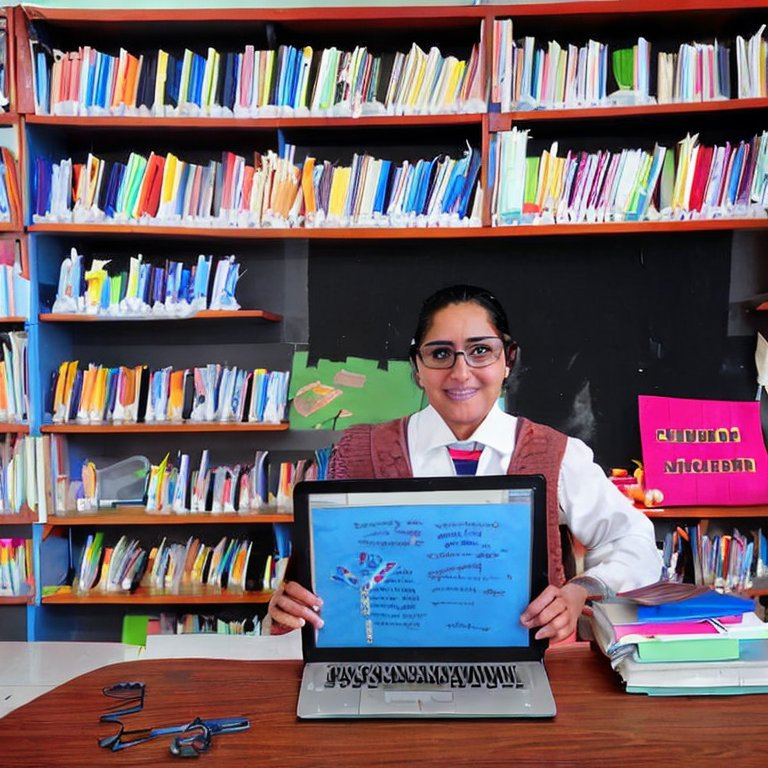
\includegraphics[width=7.5cm]{figs/sd-profe-secundaria}
    \end{column}%
    \hfill%
    \begin{column}{.38\textwidth}
      Profesor de tecnología de educación secundaria
    \end{column}%
  \end{columns}

\end{frame}

%%-----------------------------------------
\begin{frame}[fragile]

    \begin{columns}[T]
    \begin{column}{.58\textwidth}
        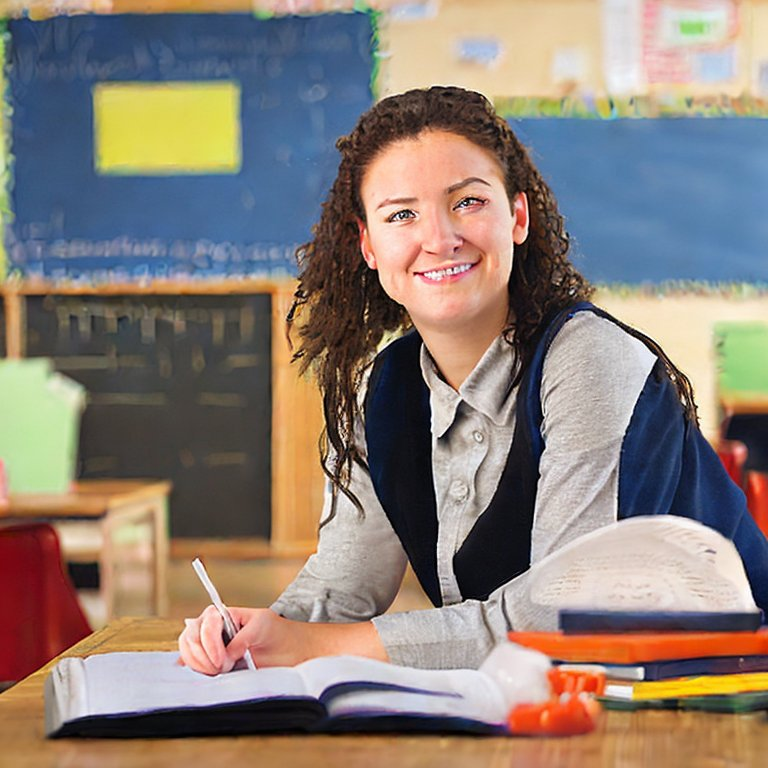
\includegraphics[width=7.5cm]{figs/sd-teacher-tech}
    \end{column}%
    \hfill%
    \begin{column}{.38\textwidth}
      Technology teacher, secondary education, portrait
    \end{column}%
  \end{columns}

\end{frame}


%%-----------------------------------------
\begin{frame}[fragile]

  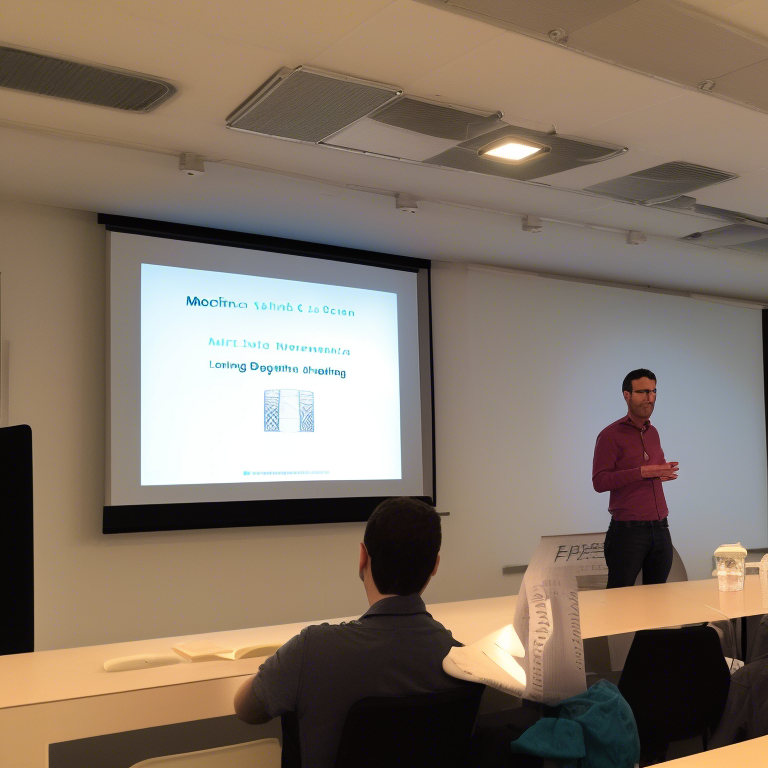
\includegraphics[width=5.5cm]{figs/sd-machine-learning-spain-25}
  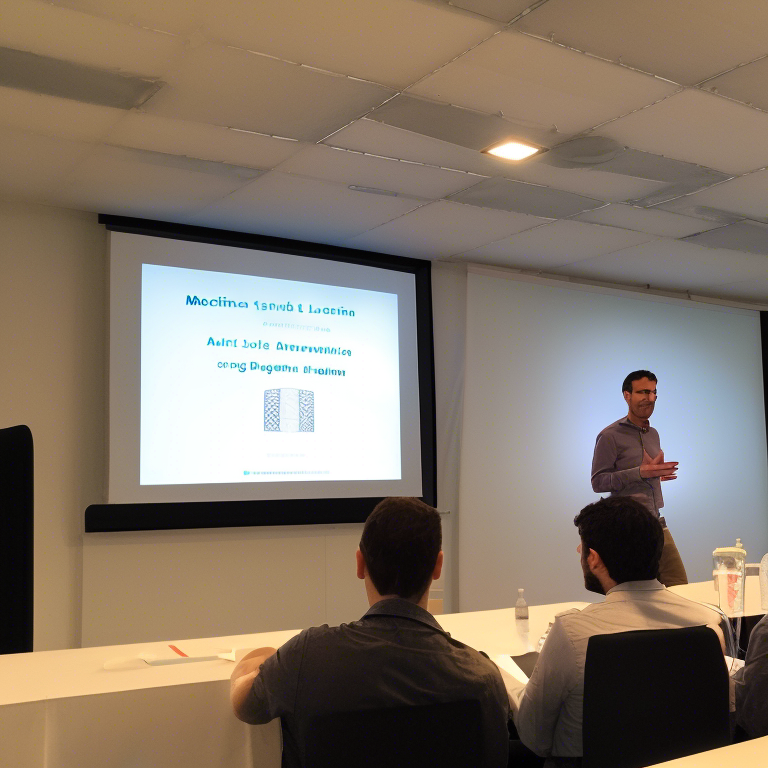
\includegraphics[width=5.5cm]{figs/sd-machine-learning-spain-50}

  {\small
  Speaker presenting at Machine Learning Spain (25, 50)
}  
\end{frame}

%%-----------------------------------------
\begin{frame}[fragile]

  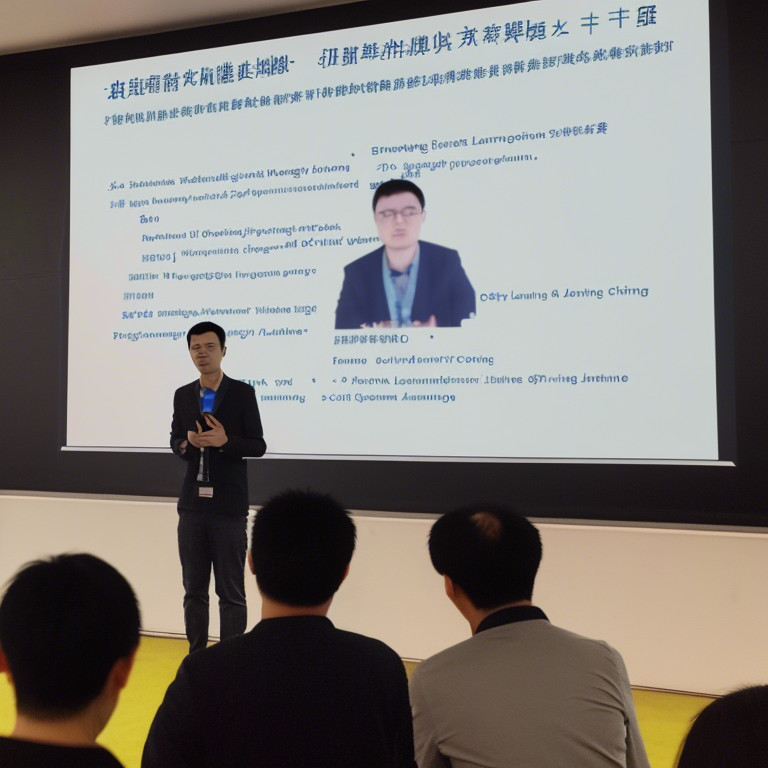
\includegraphics[width=5.5cm]{figs/sd-machine-learning-china-50}

  {\small
  Speaker presenting at Machine Learning China
}  
\end{frame}


%%-----------------------------------------
\begin{frame}[fragile]
  \frametitle{First release}

  Released on August 22nd 2022

  Licensed: Creative ML OpenRAIL-M

  \begin{flushright}
    {\scriptsize
    \url{https://stability.ai/blog/stable-diffusion-announcement} \\
    \url{https://colab.research.google.com/github/huggingface/notebooks/blob/main/diffusers/stable_diffusion.ipynb} \\
    }
  \end{flushright}
\end{frame}


%%-----------------------------------------
\begin{frame}[fragile]
  \frametitle{One week is just one week}


  Demos in Google Collab

  Model in Hugging Face

  Demonstrator available (Dream Studio)
  
  Source code and weights available
  
    \begin{flushright}
    {\scriptsize
    \url{https://multimodal.art/news/1-week-of-stable-diffusion} \\
    }
  \end{flushright}

\end{frame}

%% -----------------------------------------
\begin{frame}[fragile]
  \frametitle{Dream Studio}

  Social site to give Stable Diffusion a try \\
  Some gratis credit \\
  USD 10 for 5,000 images \\

  \begin{flushright}
    {
    \url{https://beta.dreamstudio.ai} \\
    }
  \end{flushright}
\end{frame}


%%-----------------------------------------
\begin{frame}[fragile]
  \frametitle{Stable Diffusion 2}

  Announced: November 25th 2022
  
  \begin{flushright}
    {\scriptsize
      \url{https://huggingface.co/spaces/stabilityai/stable-diffusion} \\
    }
  \end{flushright}

  Más resolución,\\ más precisión en los estilos,\\ más control.\\
\end{frame}

%% -----------------------------------------
\begin{frame}[fragile]
  \frametitle{Stable Diffusion process}

      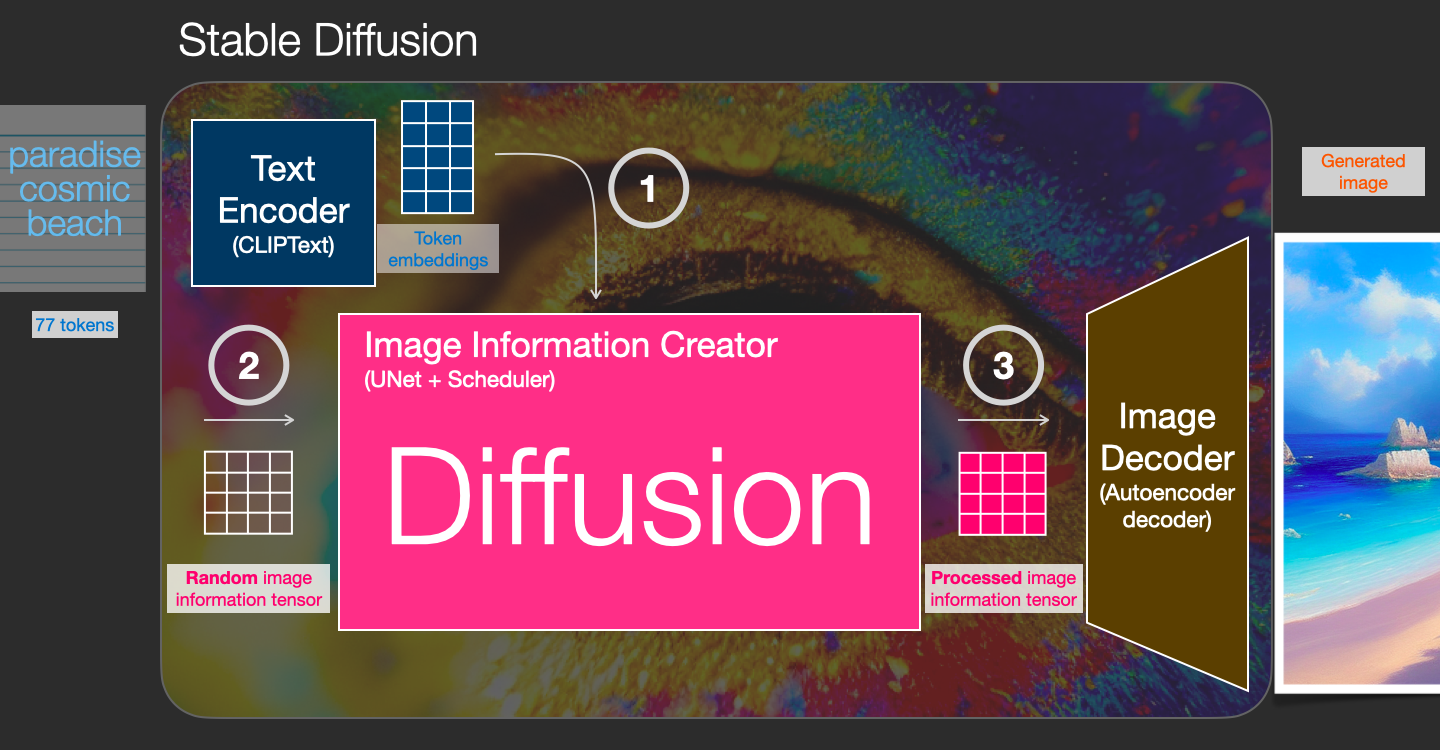
\includegraphics[width=10cm]{figs/sd-process}

  \begin{flushright}
    {\scriptsize
    \url{https://jalammar.github.io/illustrated-stable-diffusion/}
    }
  \end{flushright}

\end{frame}


%%-----------------------------------------
%%-----------------------------------------
\section{Extensions, integrations}

%%-----------------------------------------
\begin{frame}[fragile]
  \frametitle{Integration: GIMP}

    \begin{center}
    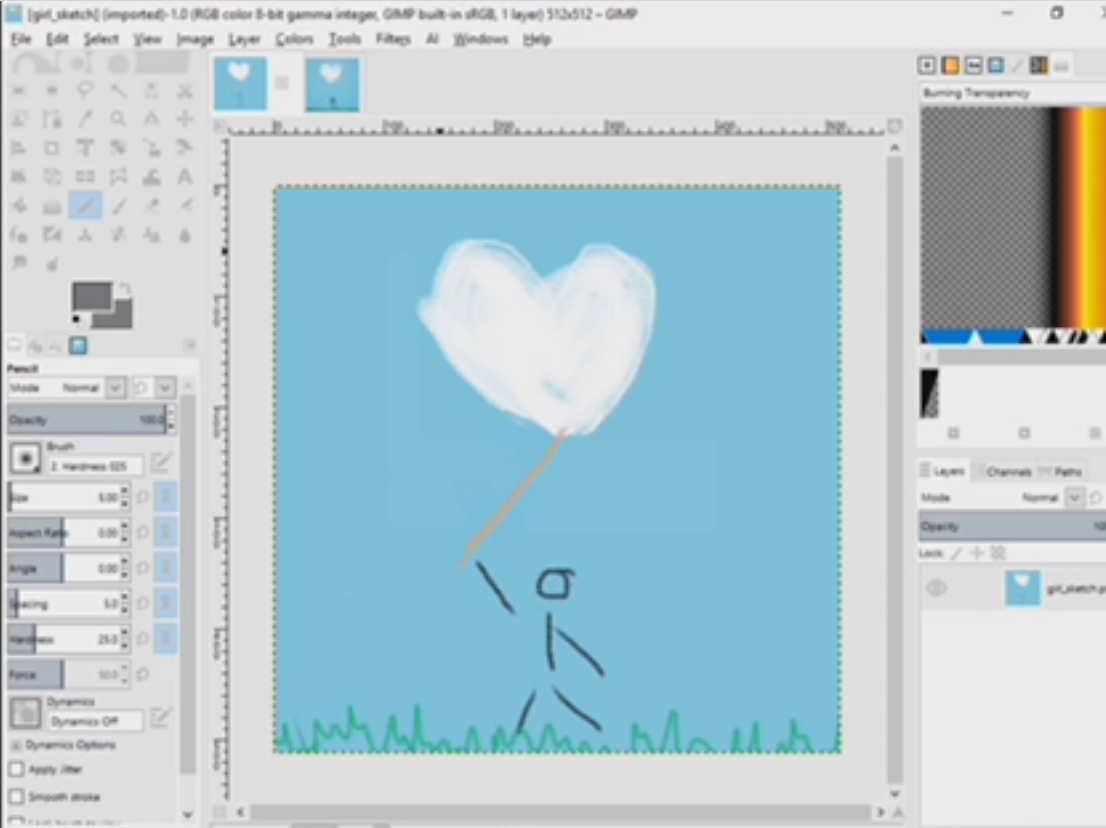
\includegraphics[width=7cm]{figs/sd-gimp}
  \end{center}

  \begin{flushright}
    {\scriptsize
    \url{https://github.com/blueturtleai/gimp-stable-diffusion} \\
    }
  \end{flushright}
  
\end{frame}

%%-----------------------------------------
\begin{frame}[fragile]
  \frametitle{Integration: Blender}

    \begin{center}
    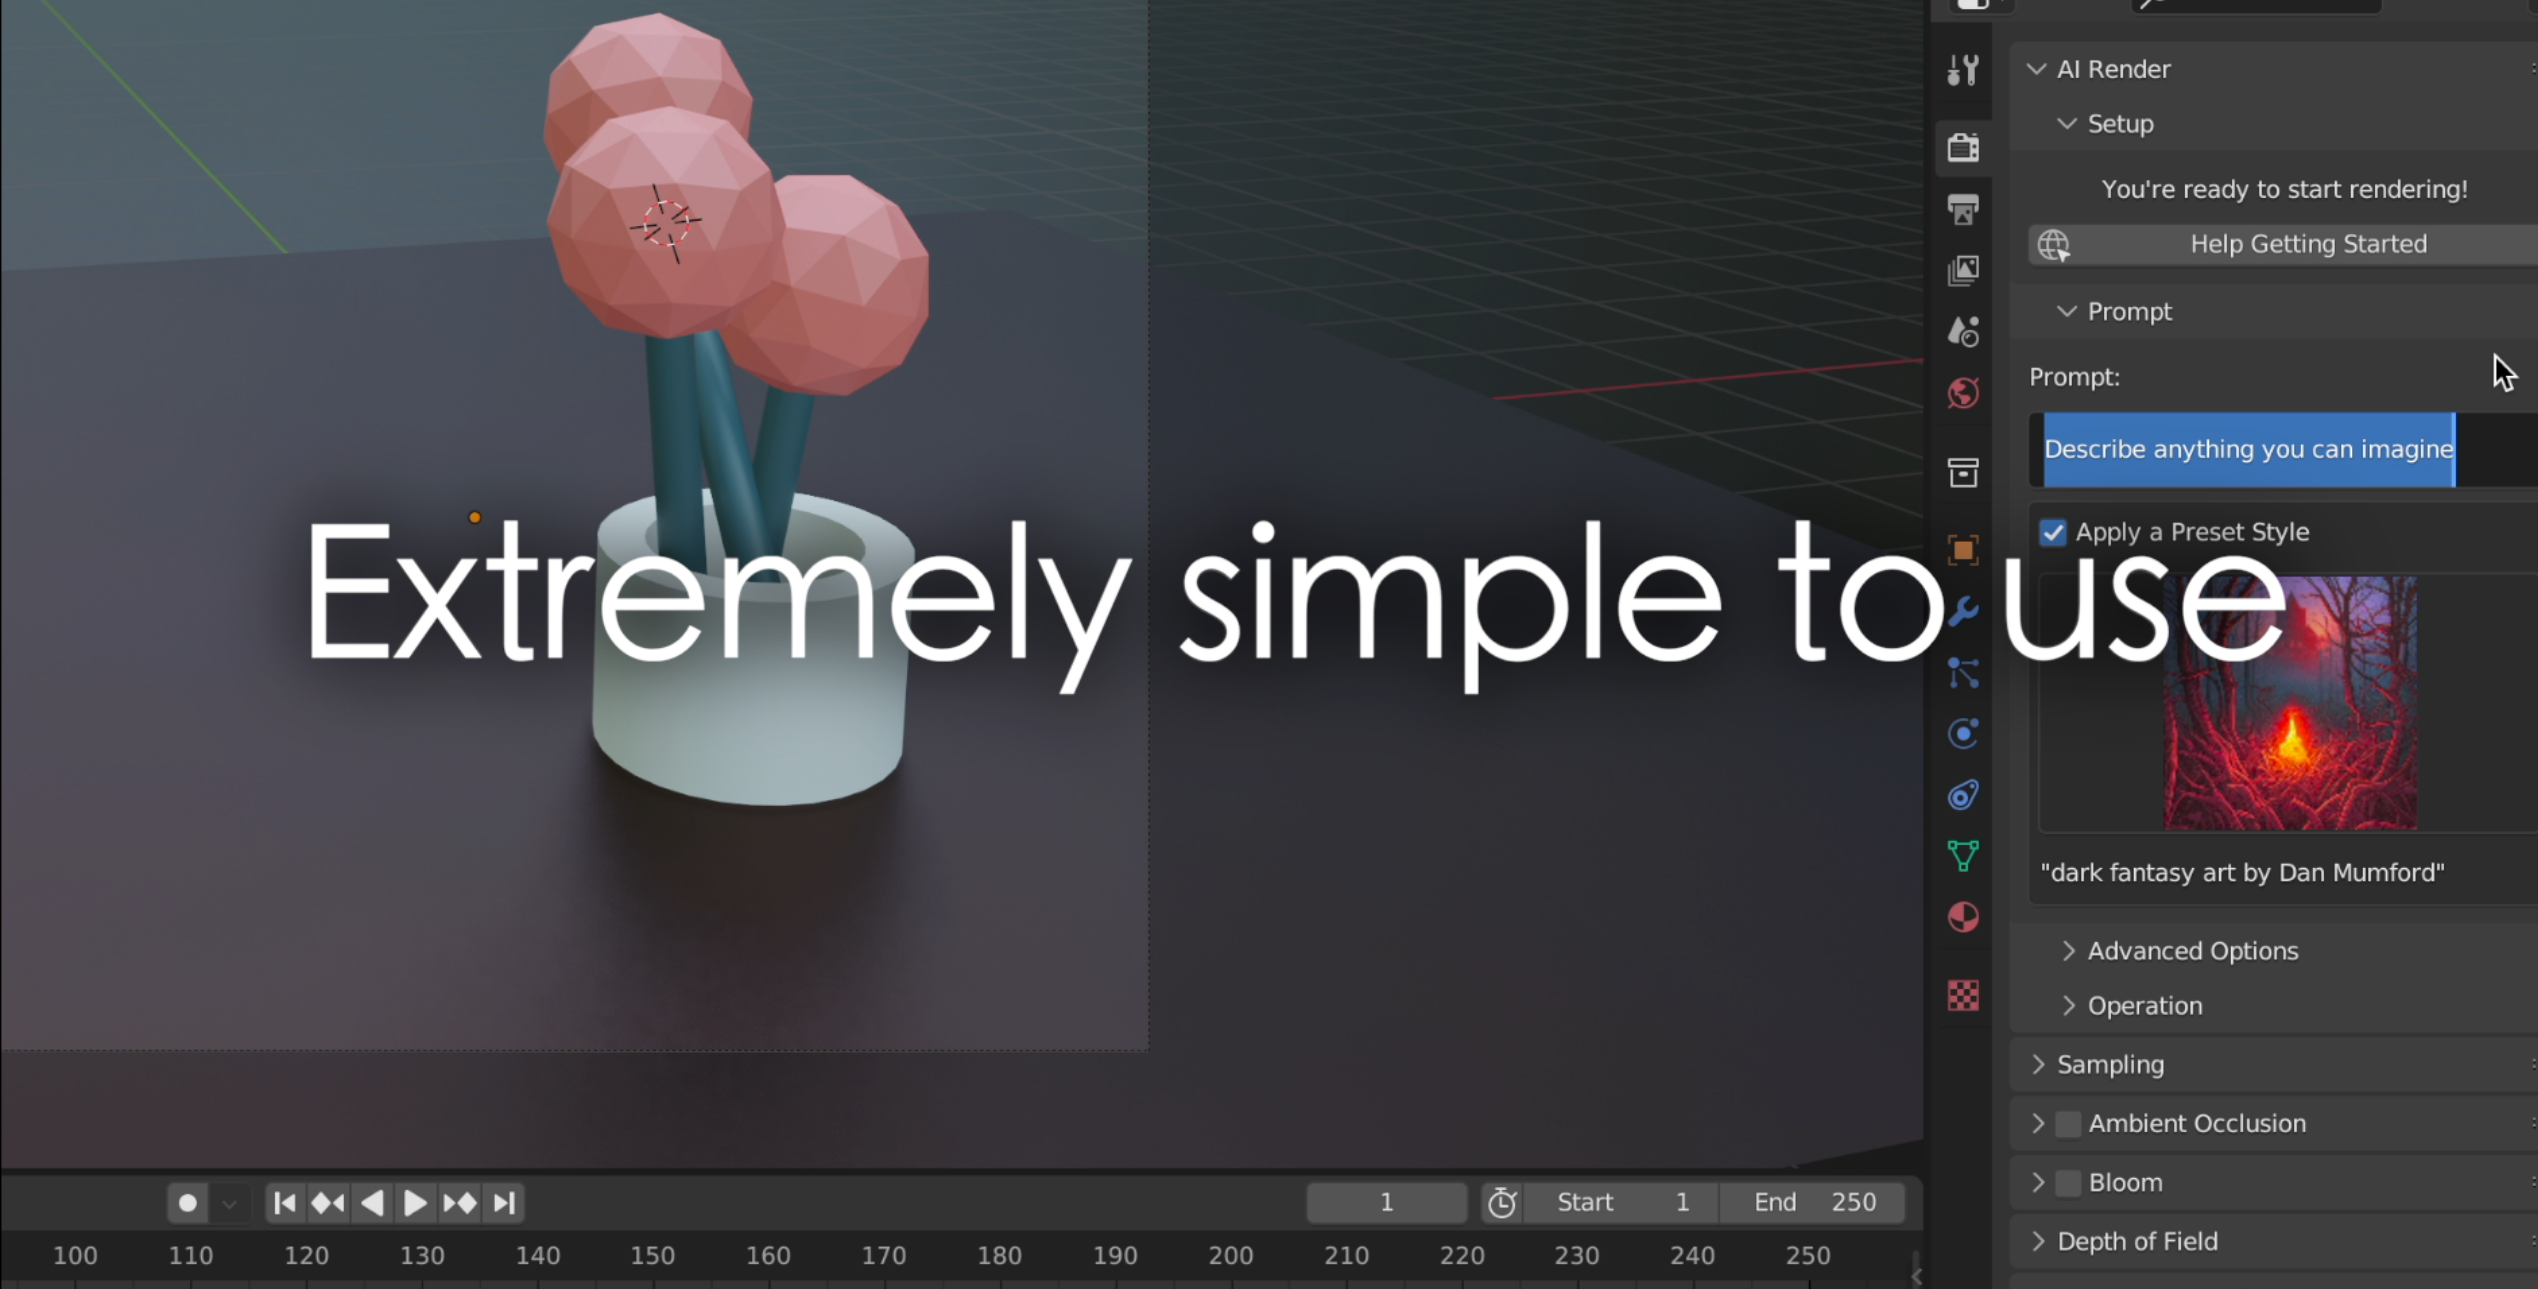
\includegraphics[width=7cm]{figs/sd-blender}
  \end{center}

  \begin{flushright}
    {\scriptsize
    \url{https://blendermarket.com/products/ai-render} \\
    }
  \end{flushright}
  
\end{frame}

%%-----------------------------------------
\begin{frame}[fragile]
  \frametitle{In-painting}

    \begin{center}
    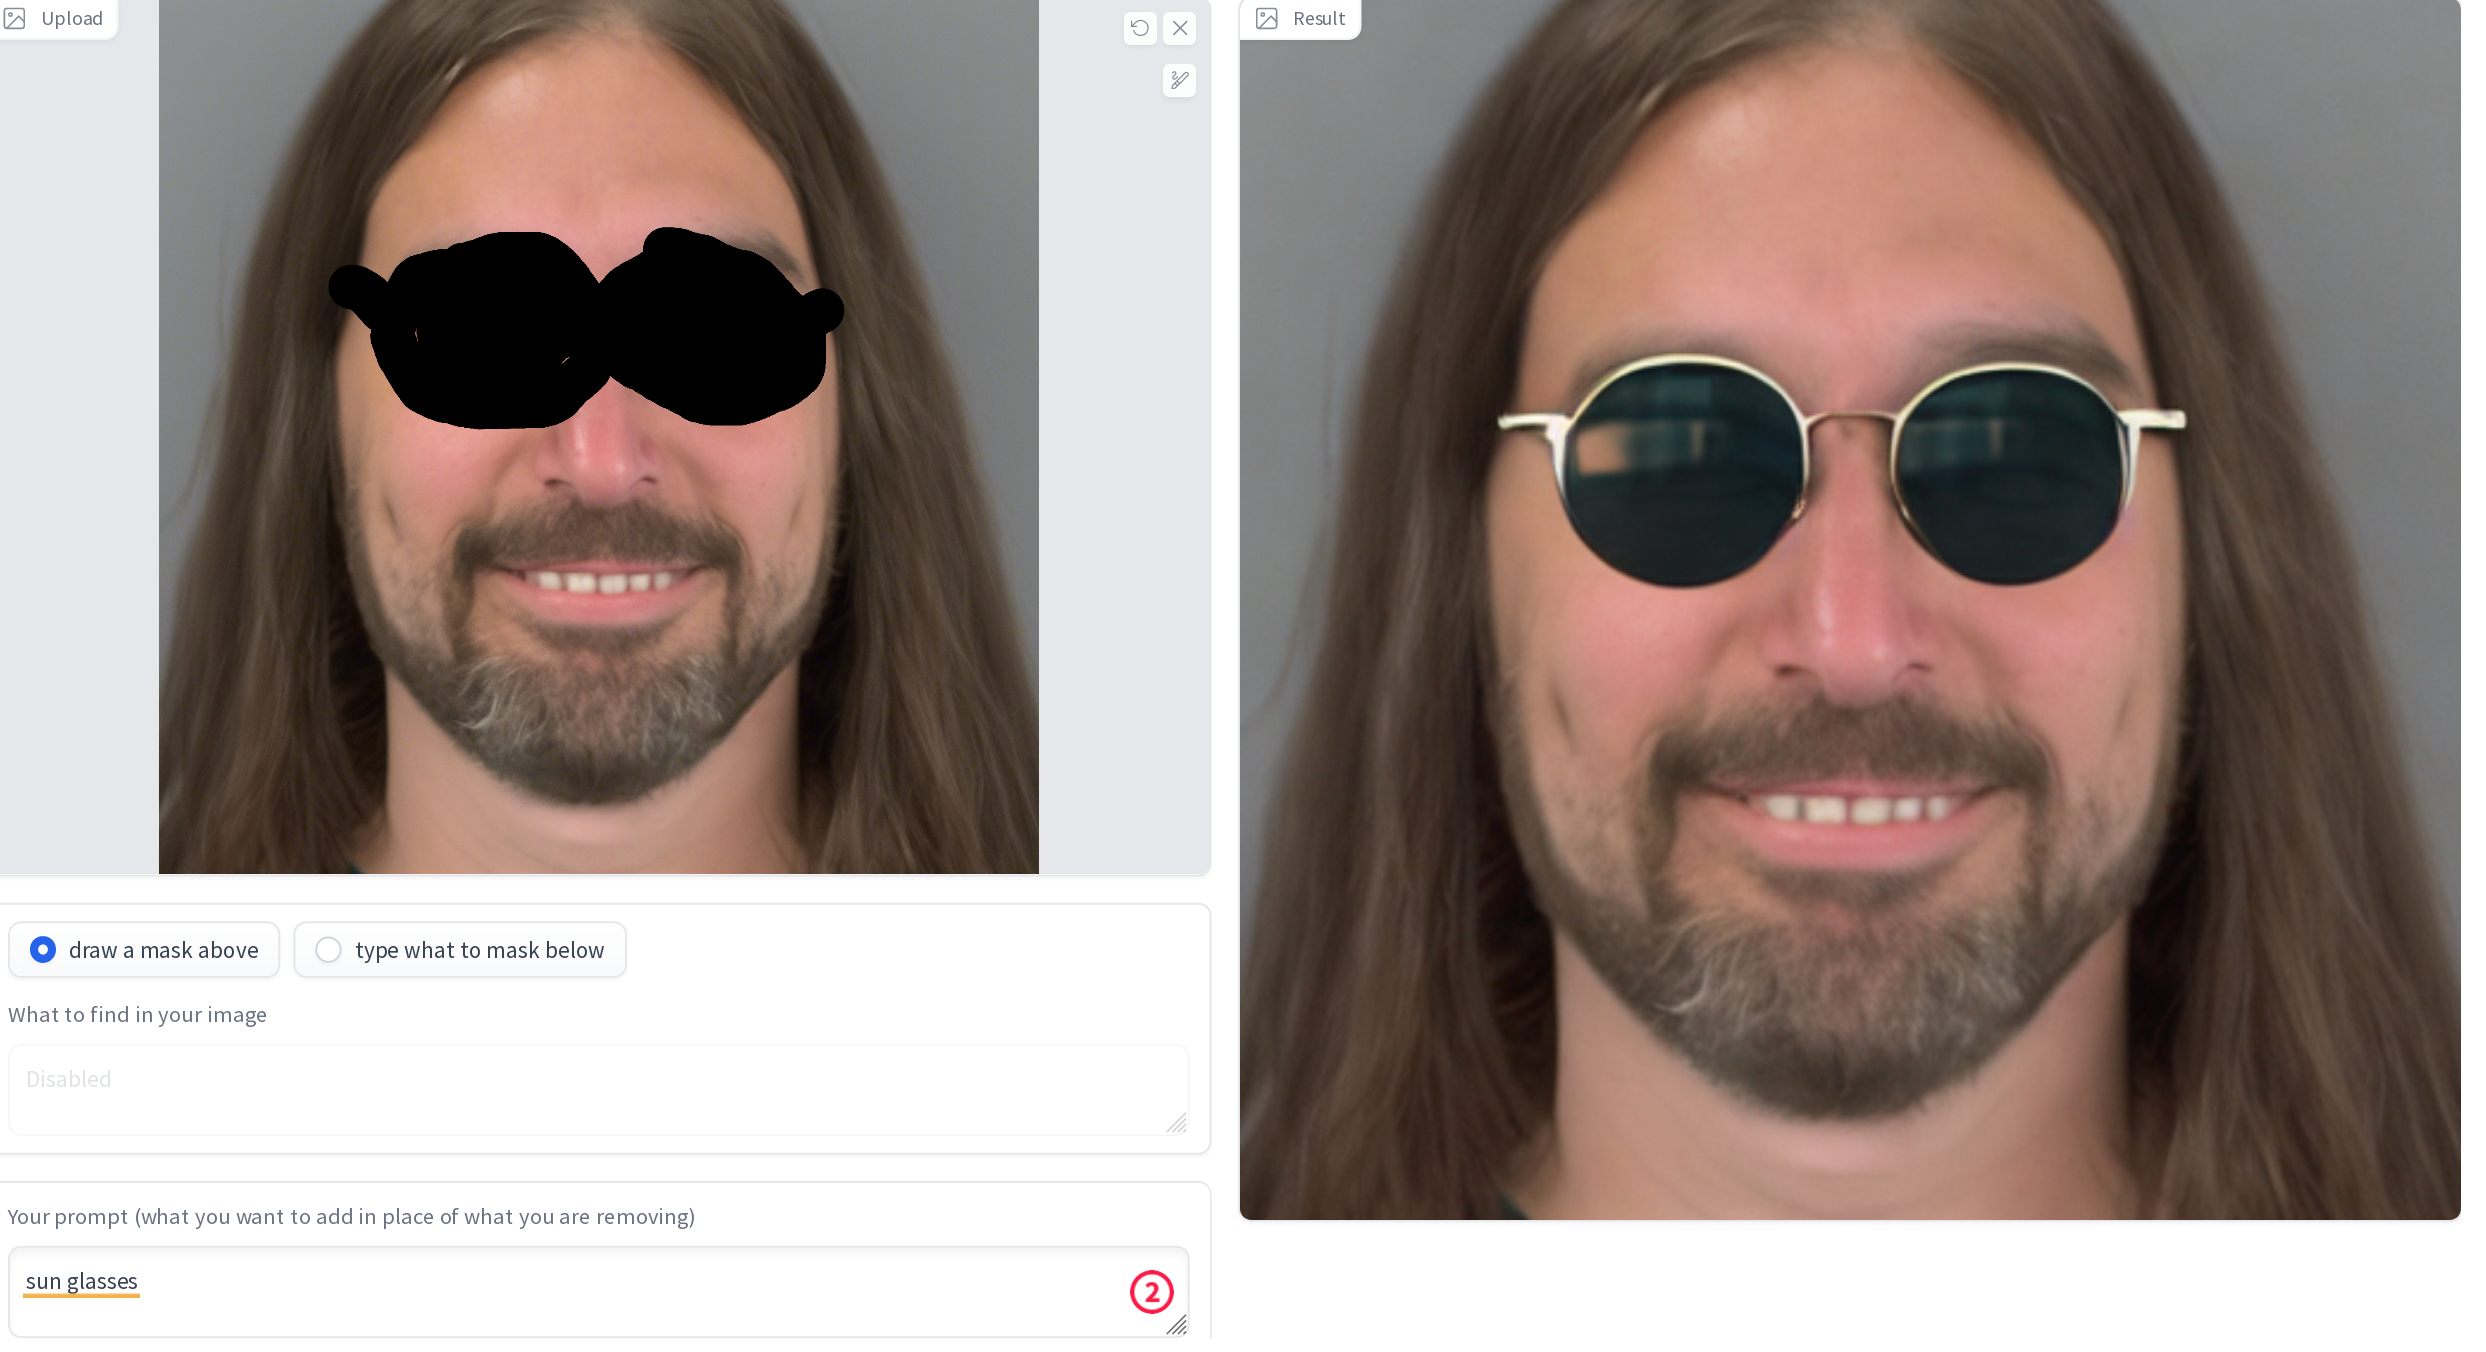
\includegraphics[width=9.5cm]{figs/sd-inpainting}
  \end{center}

  \begin{flushright}
    {\scriptsize
    \url{https://huggingface.co/spaces/multimodalart/stable-diffusion-inpainting} \\
    }
  \end{flushright}
  
\end{frame}

%%-----------------------------------------
\begin{frame}[fragile]
  \frametitle{Out-painting}

    \begin{center}
    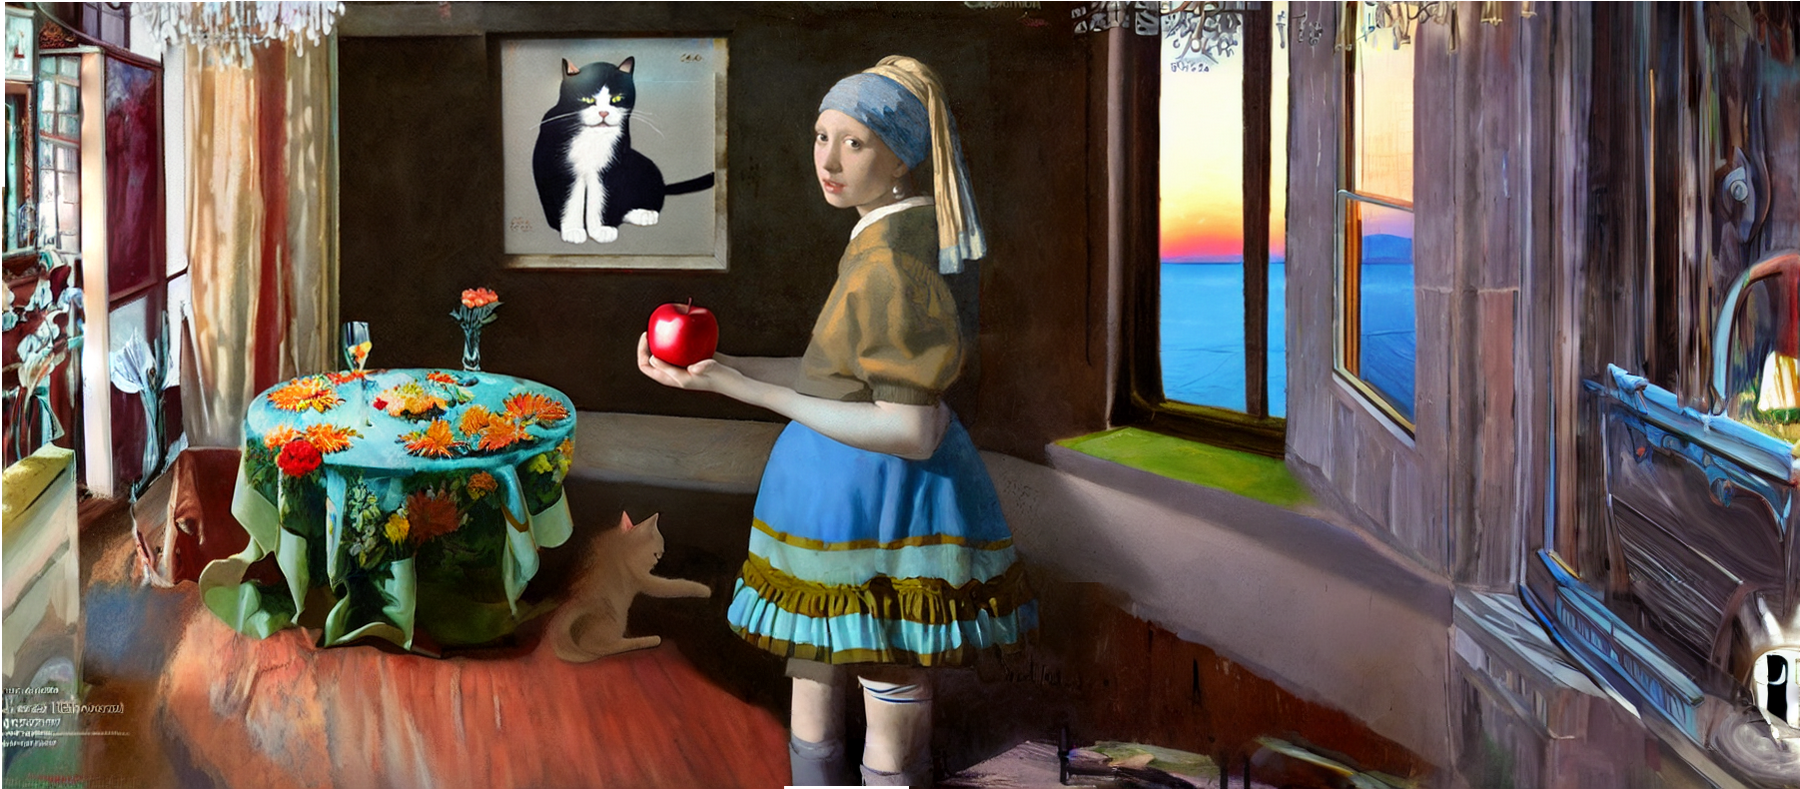
\includegraphics[width=9.5cm]{figs/sd-infinity}
  \end{center}

  \begin{flushright}
    {\scriptsize
    \url{https://github.com/lkwq007/stablediffusion-infinity} \\
    }
  \end{flushright}


  
  
\end{frame}


%% -----------------------------------------
\begin{frame}[fragile]
  \frametitle{Image to image}

  Image + prompt produces an image \\
  Even just with CPU! \\
  
  \begin{flushright}
    {\scriptsize
    \url{https://huggingface.co/spaces/fffiloni/stable-diffusion-img2img} \\
    }
  \end{flushright}
  
\end{frame}

%%-----------------------------------------
\begin{frame}[fragile]

  \begin{center}
    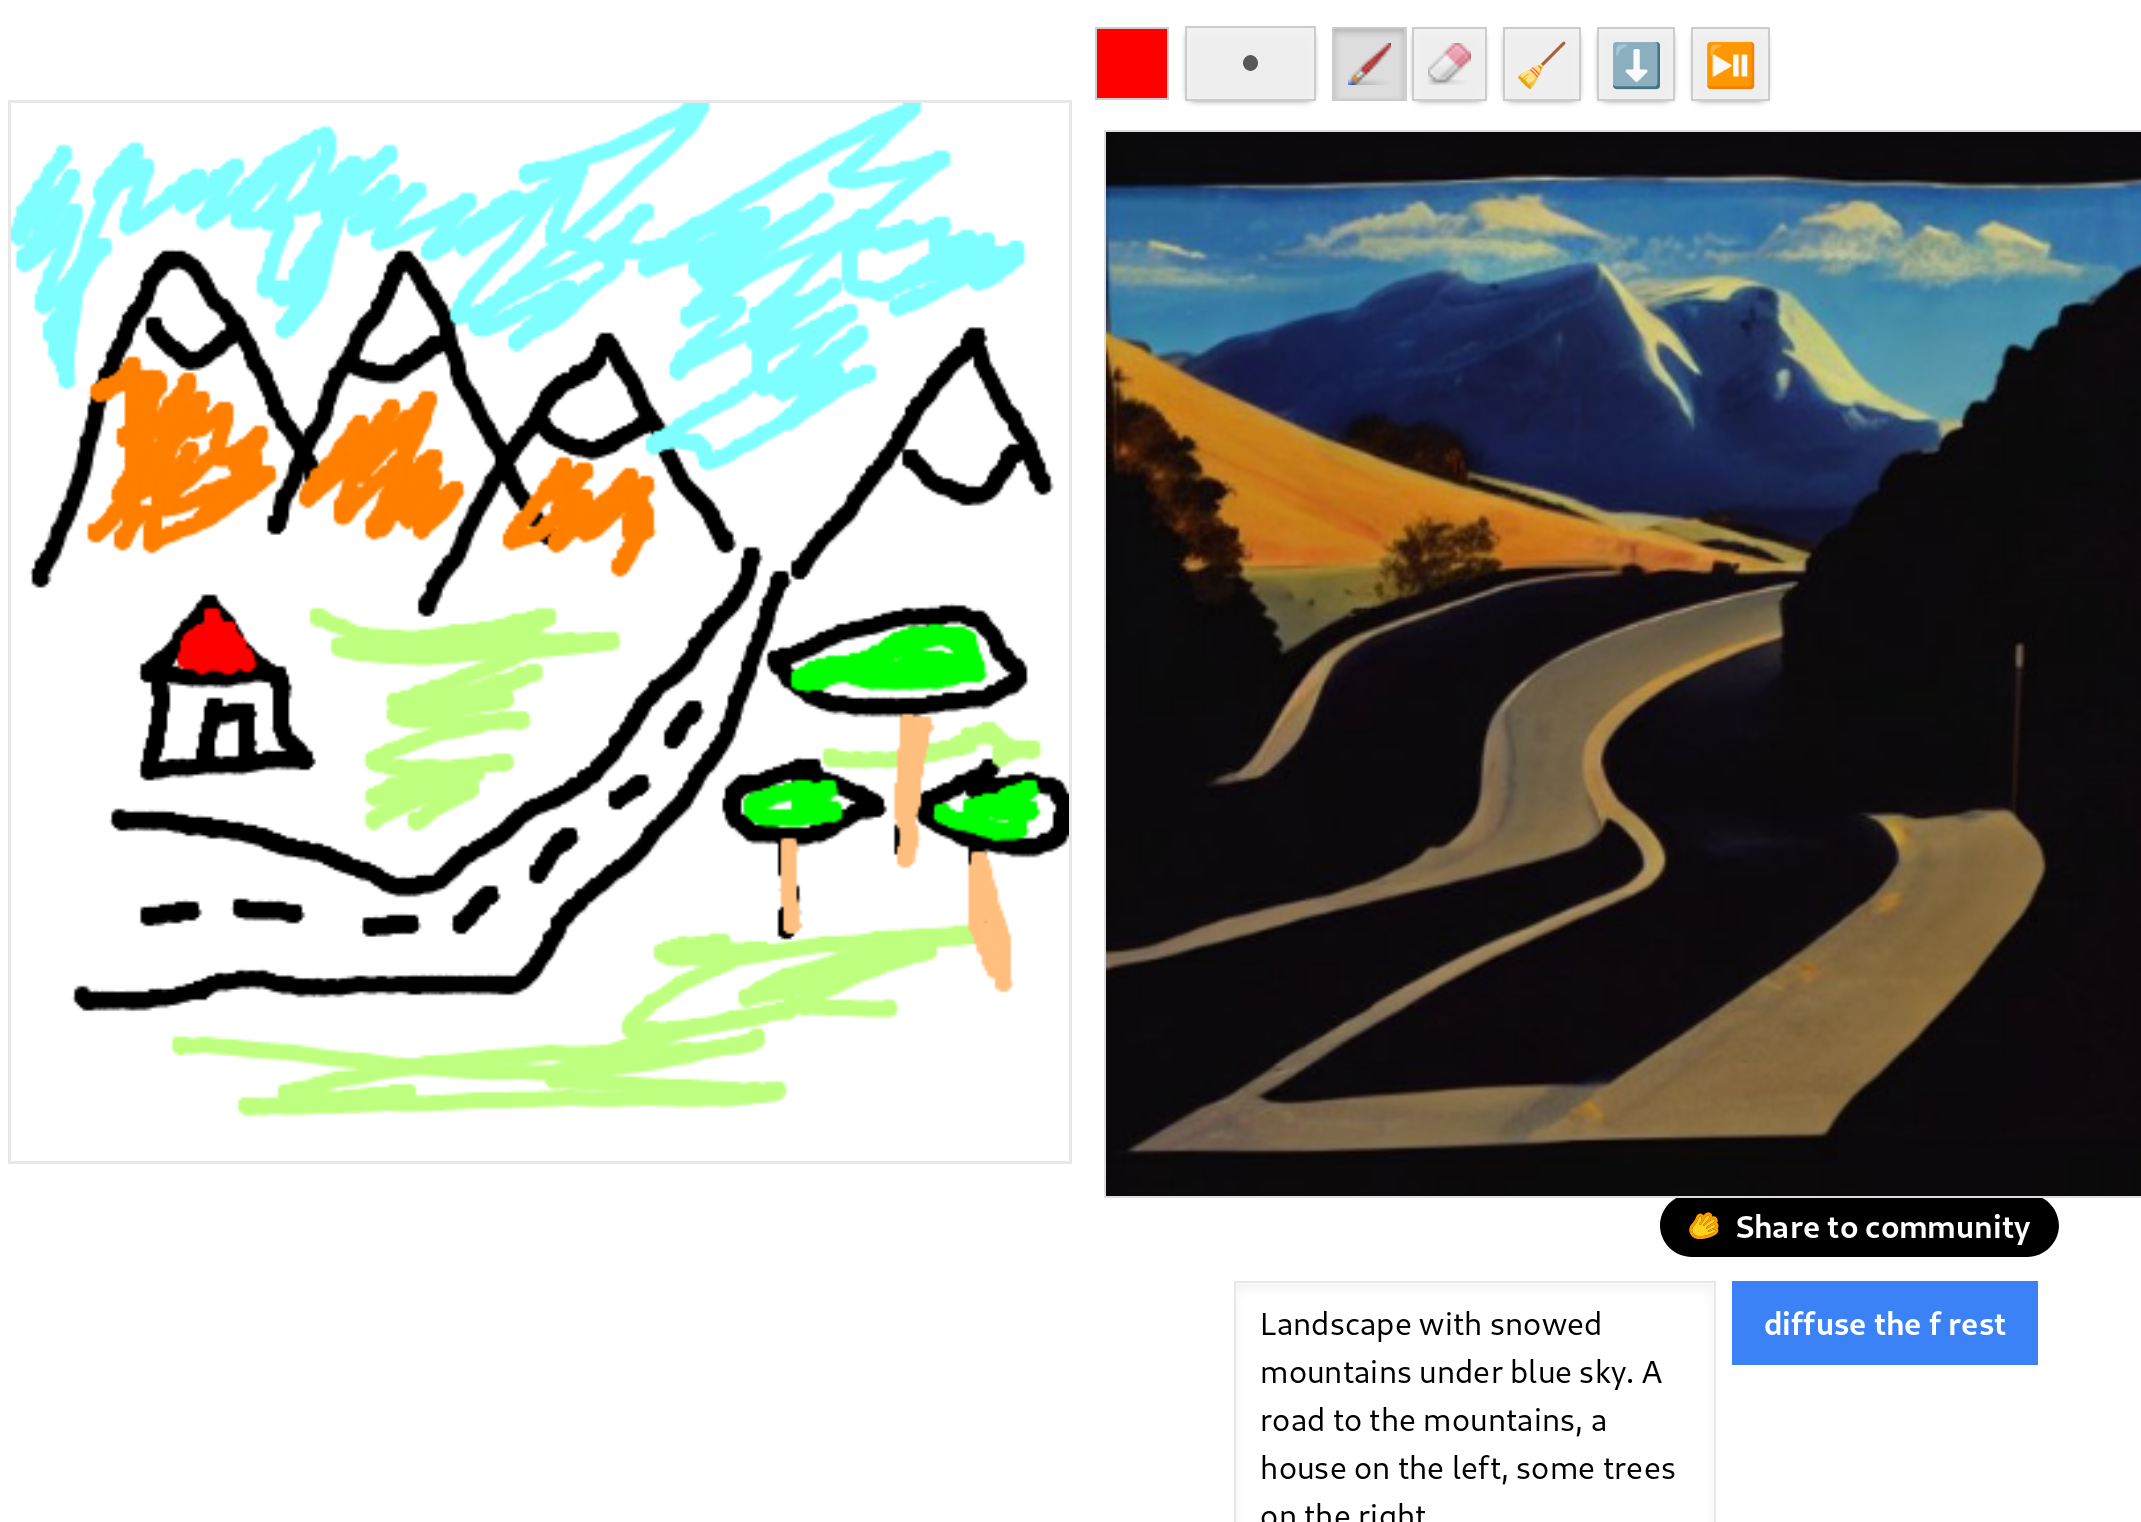
\includegraphics[width=9.5cm]{figs/sd-mountains}
  \end{center}

  \begin{flushright}
    {\scriptsize
    \url{https://huggingface.co/spaces/huggingface-projects/diffuse-the-rest} \\
    }
  \end{flushright}
    
\end{frame}

%%-----------------------------------------
\begin{frame}[fragile]
  \frametitle{Fine-tuned images}

  \begin{columns}[T]
    \begin{column}{.48\textwidth}
        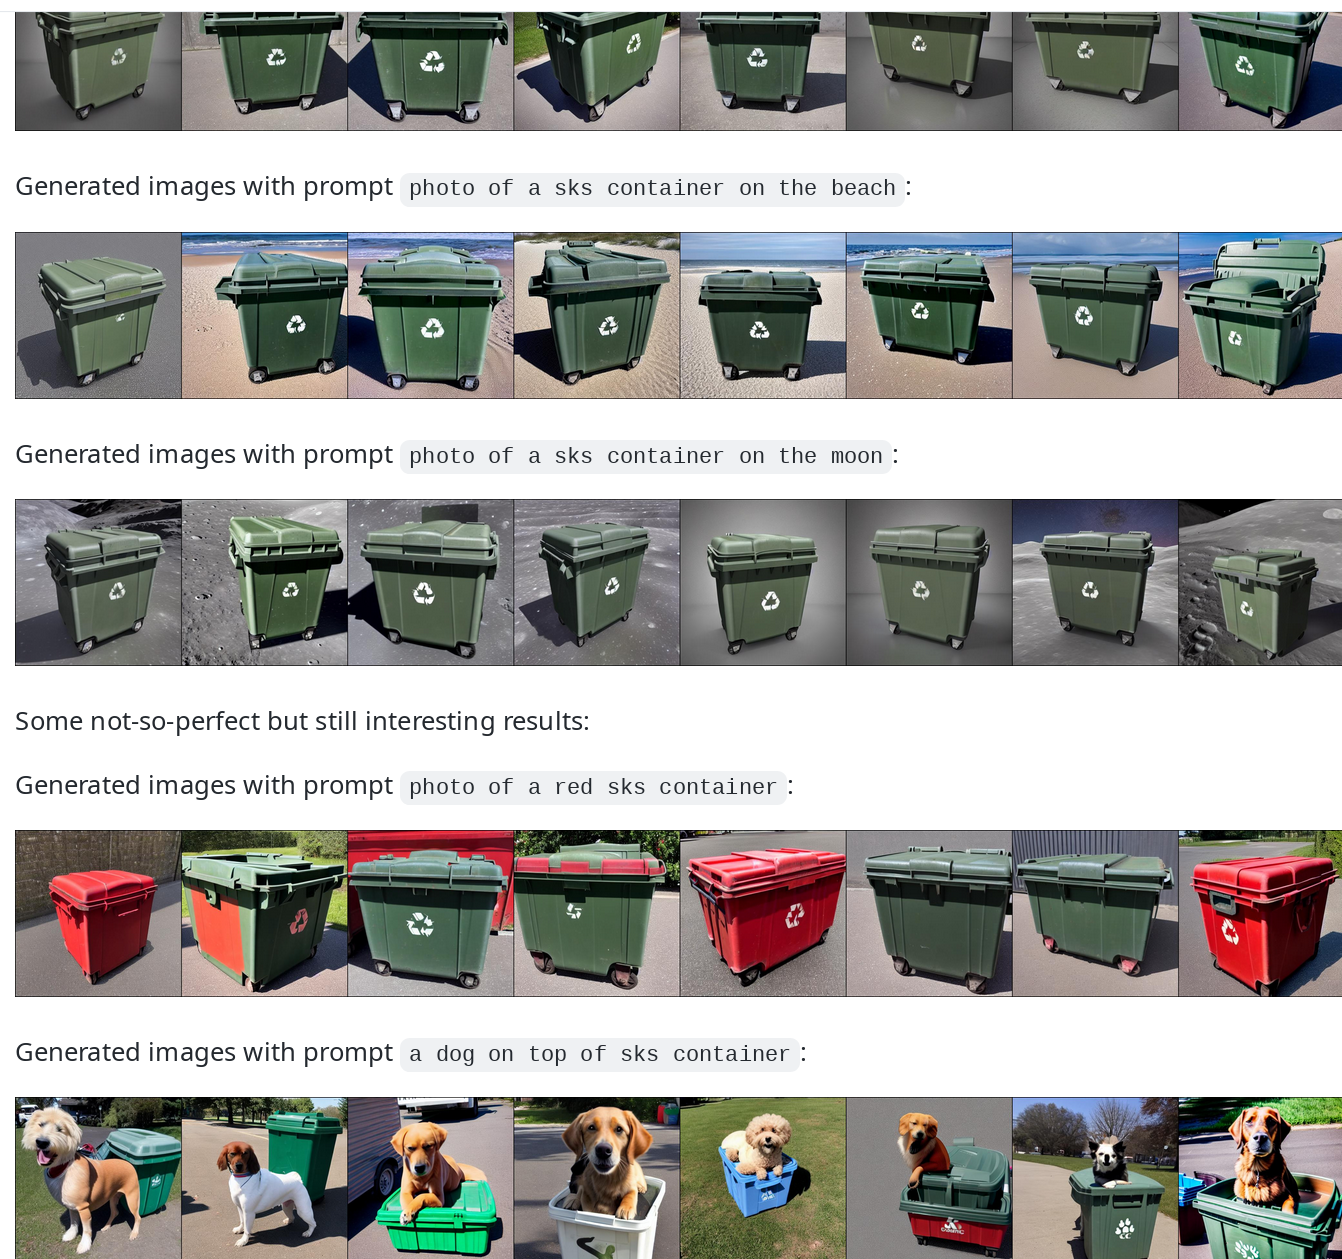
\includegraphics[width=6cm]{figs/sd-dreambooth}
    \end{column}%
    \hfill%
    \begin{column}{.48\textwidth}
      \vspace{1.5cm}
      {\scriptsize
        \url{https://github.com/XavierXiao/Dreambooth-Stable-Diffusion} \\
      }
    \end{column}%
  \end{columns}


\end{frame}

%%-----------------------------------------
\begin{frame}[fragile]
  \frametitle{3D assets}

  \begin{center}
    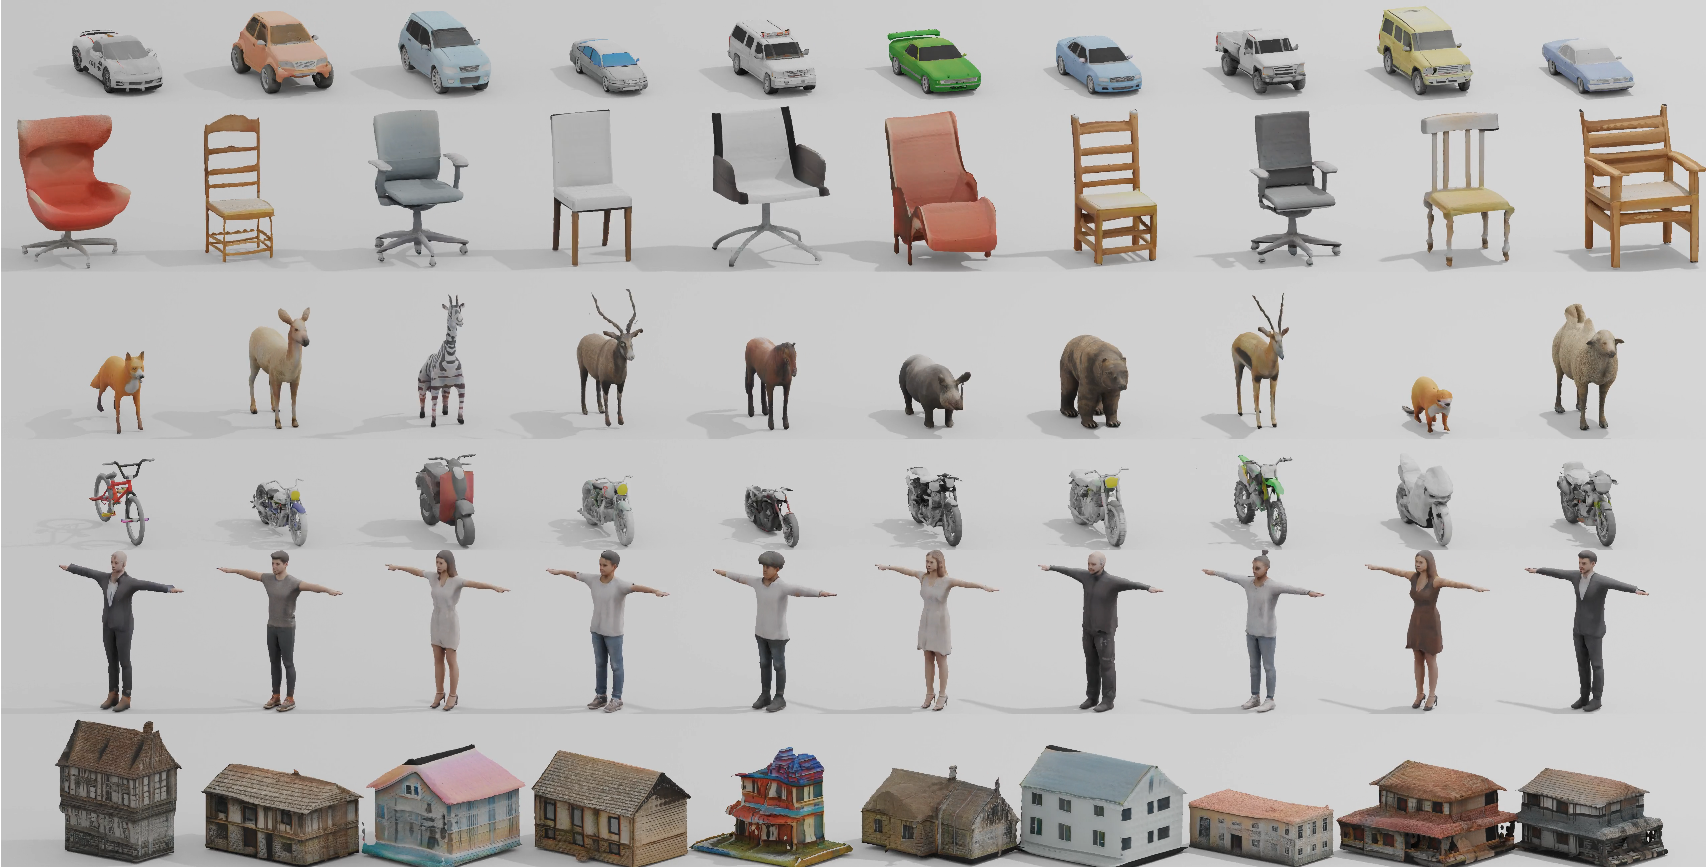
\includegraphics[width=9.5cm]{figs/get3d}
  \end{center}

  \begin{flushright}
    {\scriptsize
    \url{https://nv-tlabs.github.io/GET3D/} \\
    }
  \end{flushright}
  
\end{frame}

%%-----------------------------------------
\begin{frame}[fragile]
  \frametitle{3D assets}

  \begin{center}
    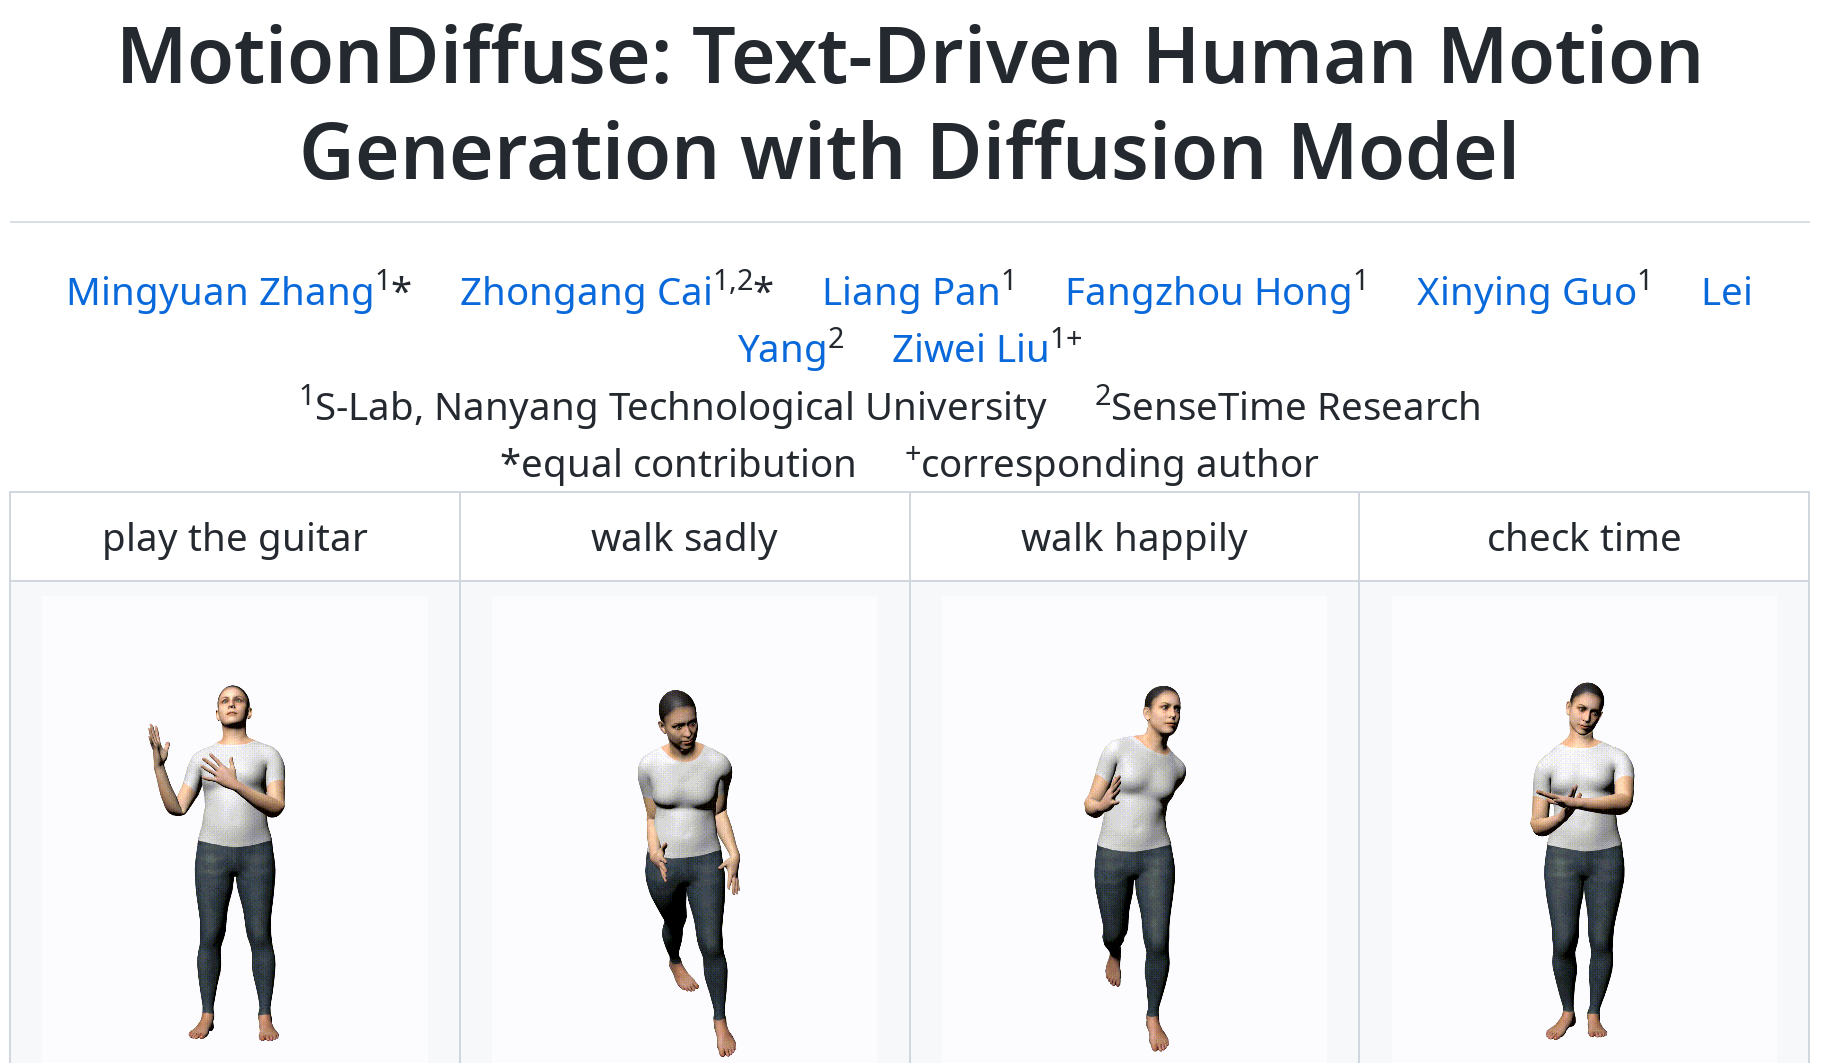
\includegraphics[width=9.5cm]{figs/human-motion}
  \end{center}

  \begin{flushright}
    {\scriptsize
    \url{https://github.com/mingyuan-zhang/MotionDiffuse} \\
    }
  \end{flushright}
  
\end{frame}

%%-----------------------------------------
\begin{frame}[fragile]
  \frametitle{Videos}

  \begin{center}
    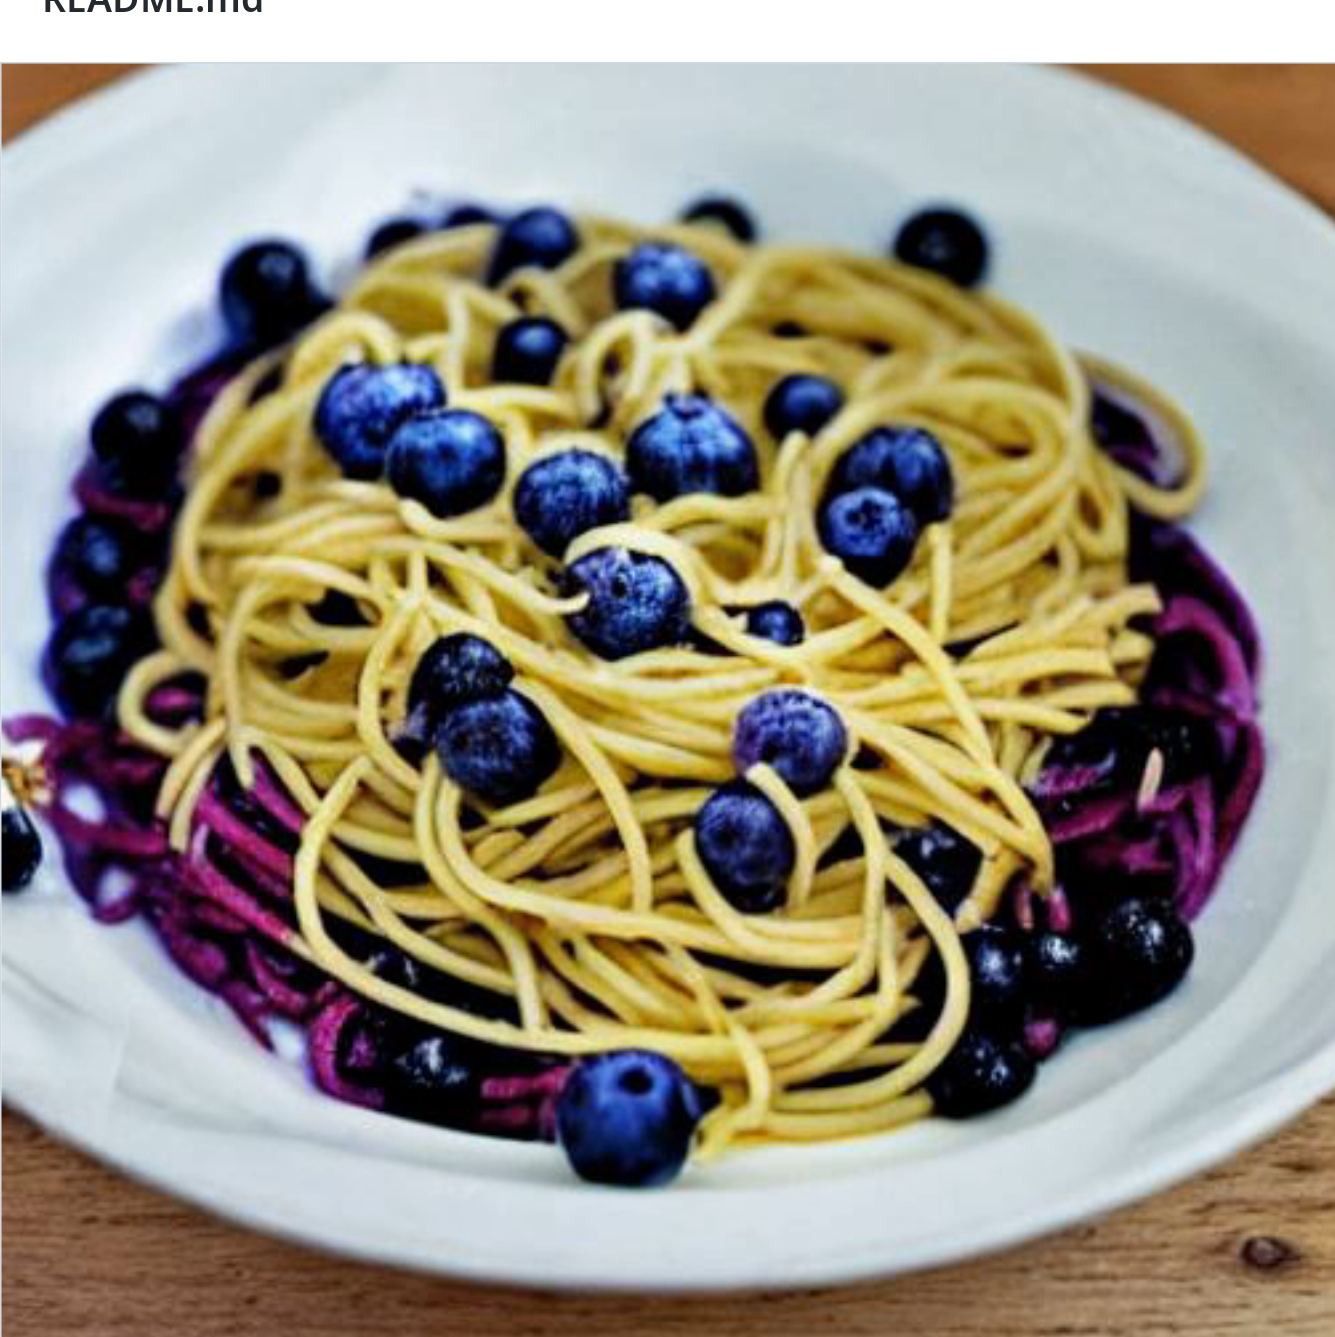
\includegraphics[width=2.5cm]{figs/sd-video-1}
    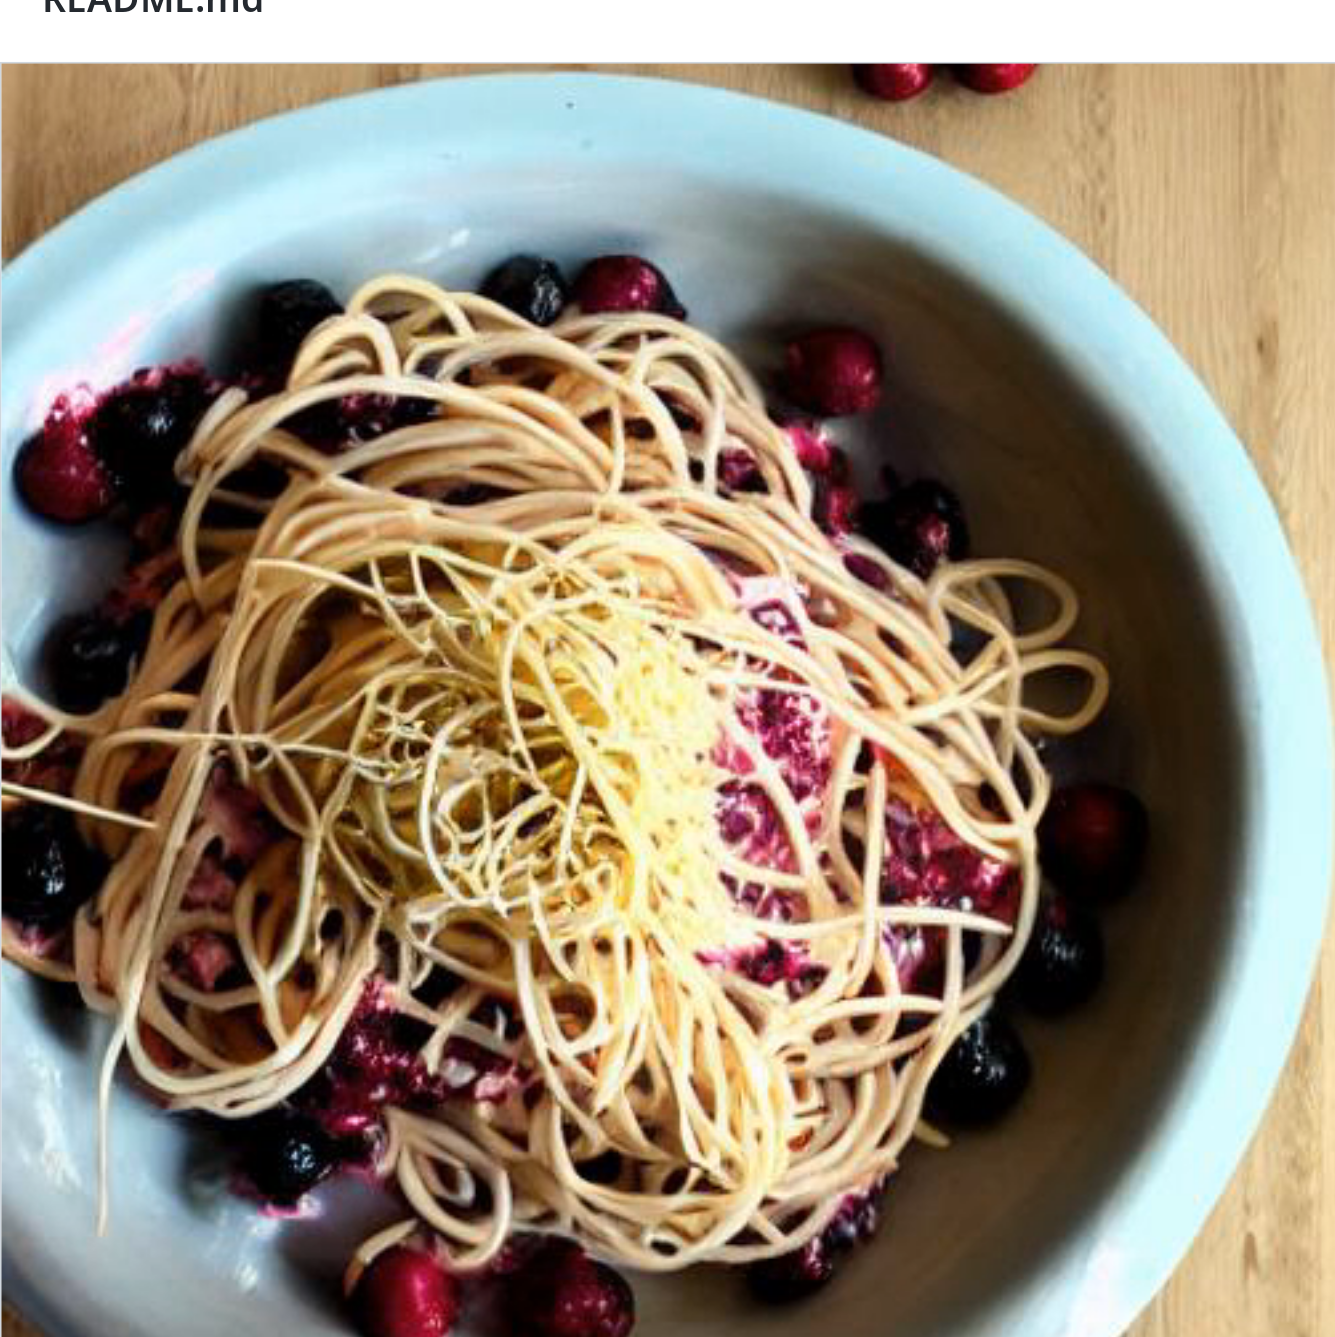
\includegraphics[width=2.5cm]{figs/sd-video-2}
    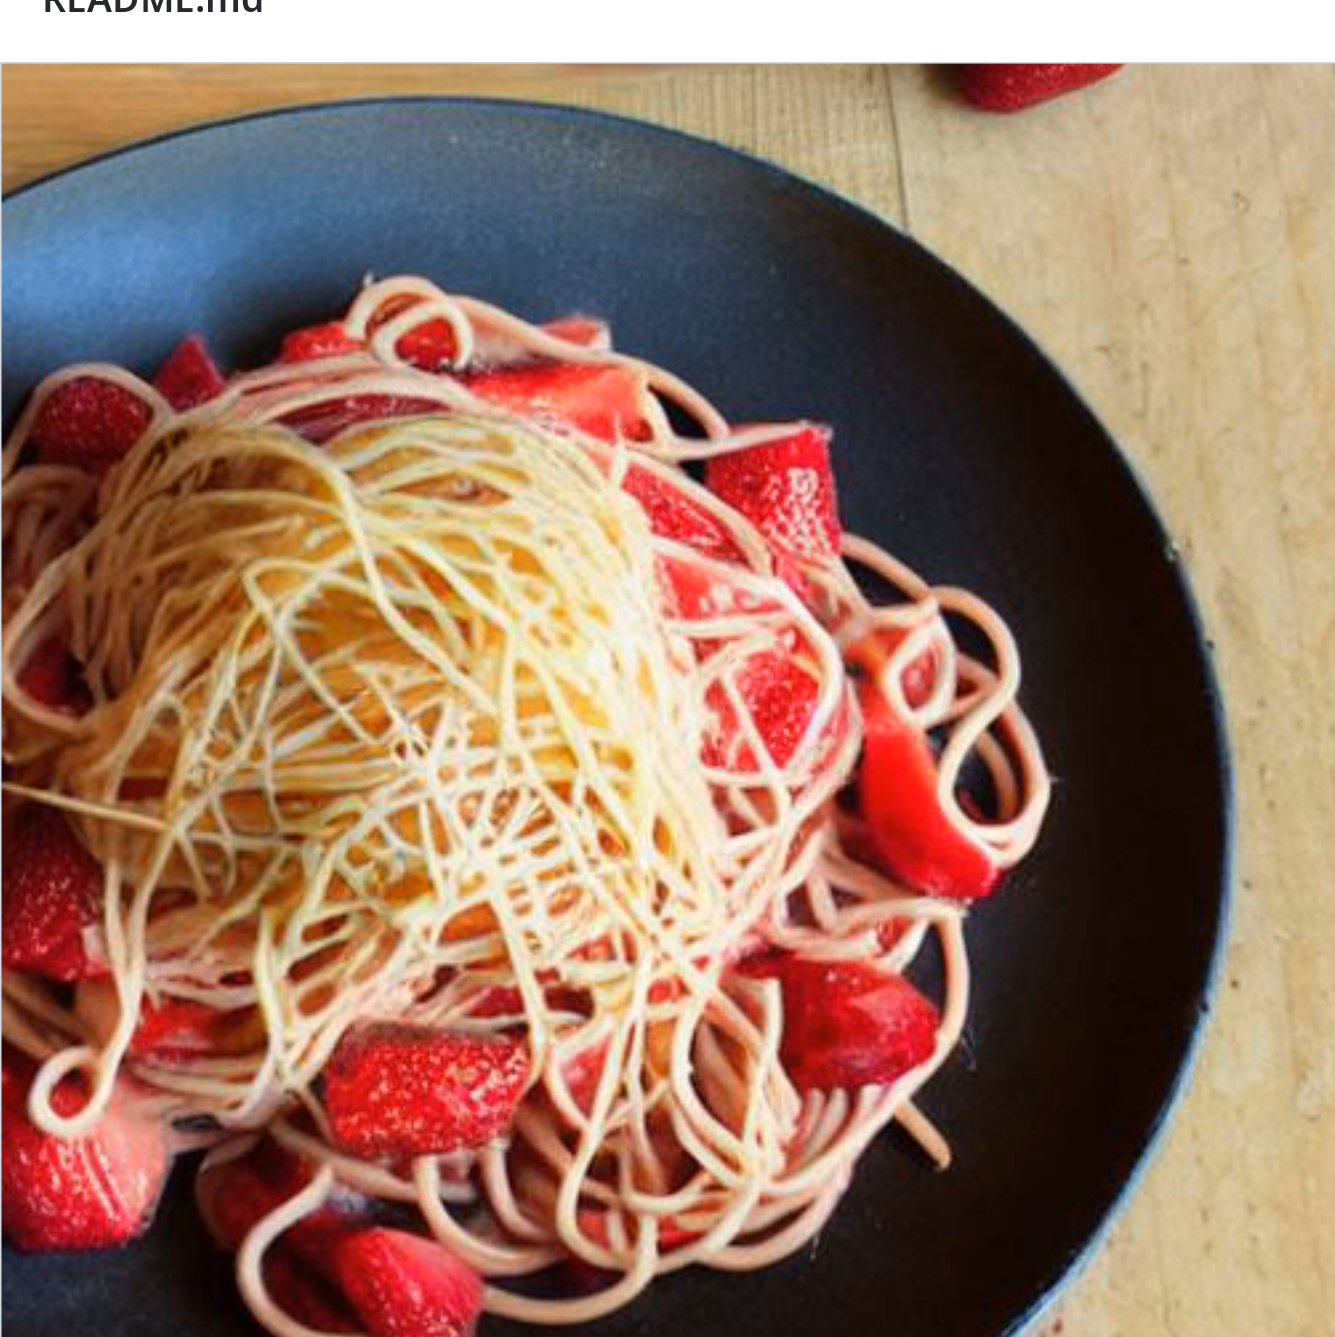
\includegraphics[width=2.5cm]{figs/sd-video-3}
    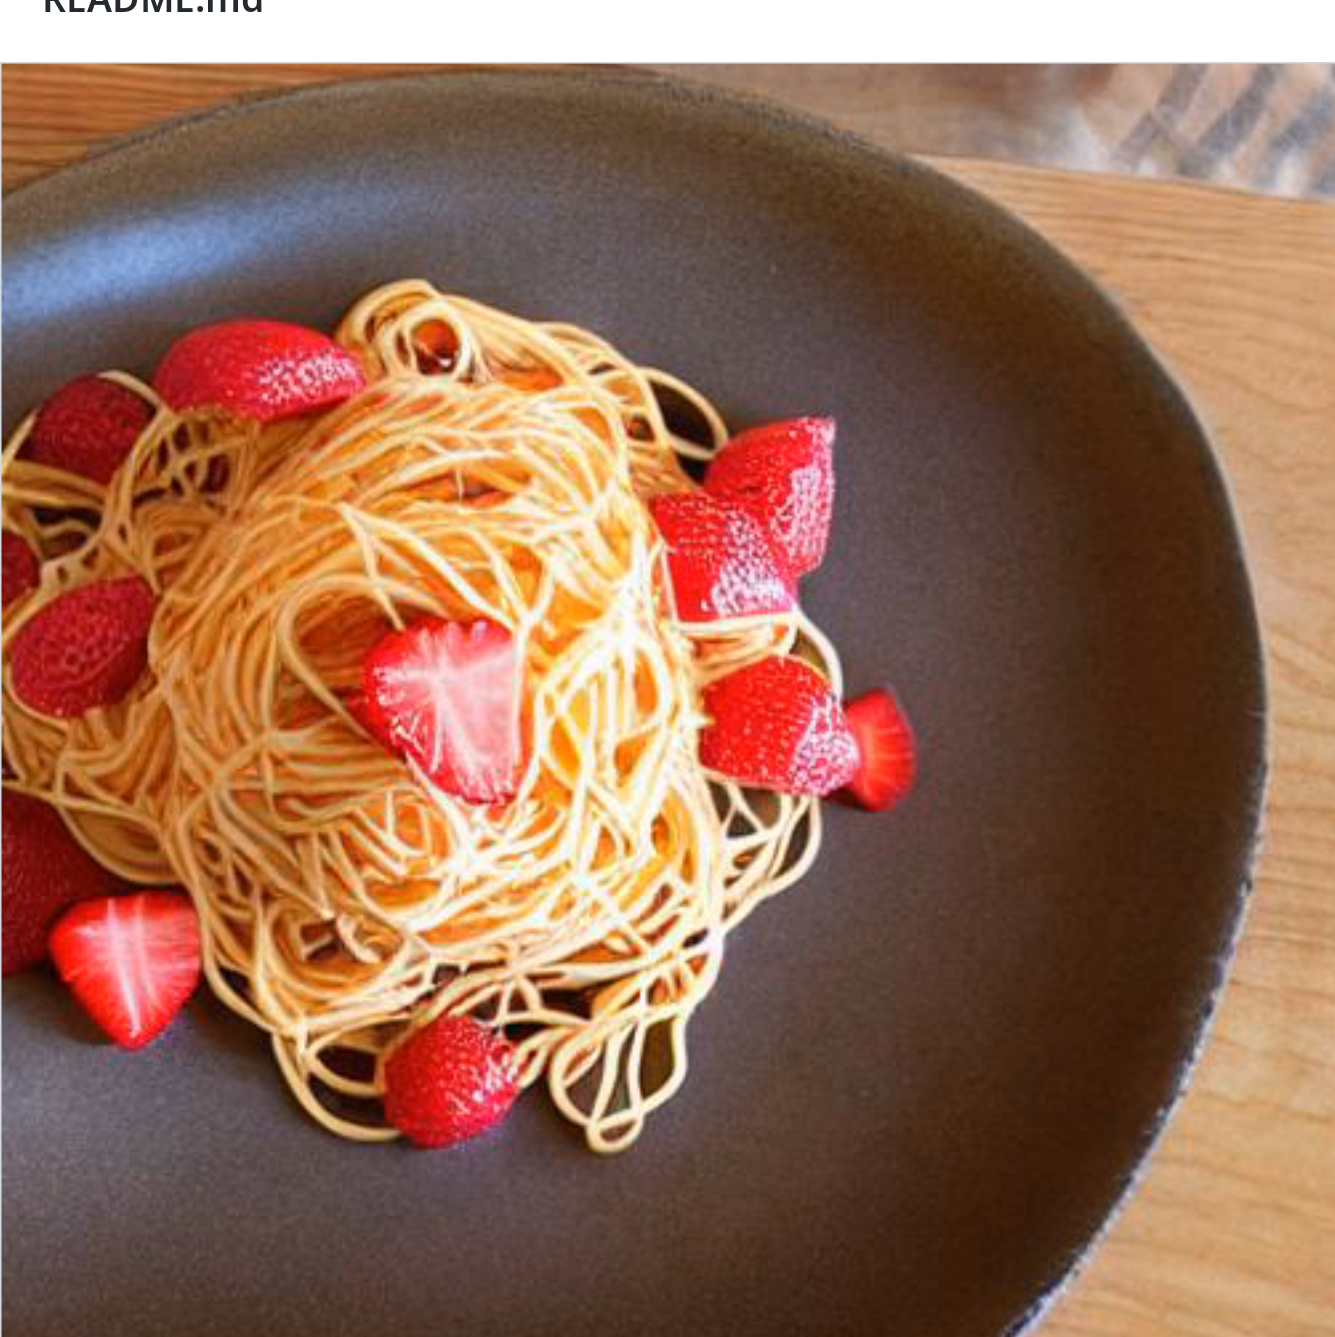
\includegraphics[width=2.5cm]{figs/sd-video-4}
  \end{center}
  
  \begin{flushright}
    {\scriptsize
      \url{https://github.com/nateraw/stable-diffusion-videos} \\
      \url{https://phenaki.github.io/} \\
      \url{https://aiart.dev/posts/sd-music-videos/sd_music_videos.html} \\
    }
  \end{flushright}
  
  
\end{frame}

%%-----------------------------------------
\begin{frame}[fragile]

  \begin{center}
    {\Large And much, much more}
  \end{center}
    
\end{frame}

%%-----------------------------------------
%%-----------------------------------------
\section{Stable Diffusion is not alone}

%%-----------------------------------------
\begin{frame}[fragile]
  \frametitle{Whisper}

  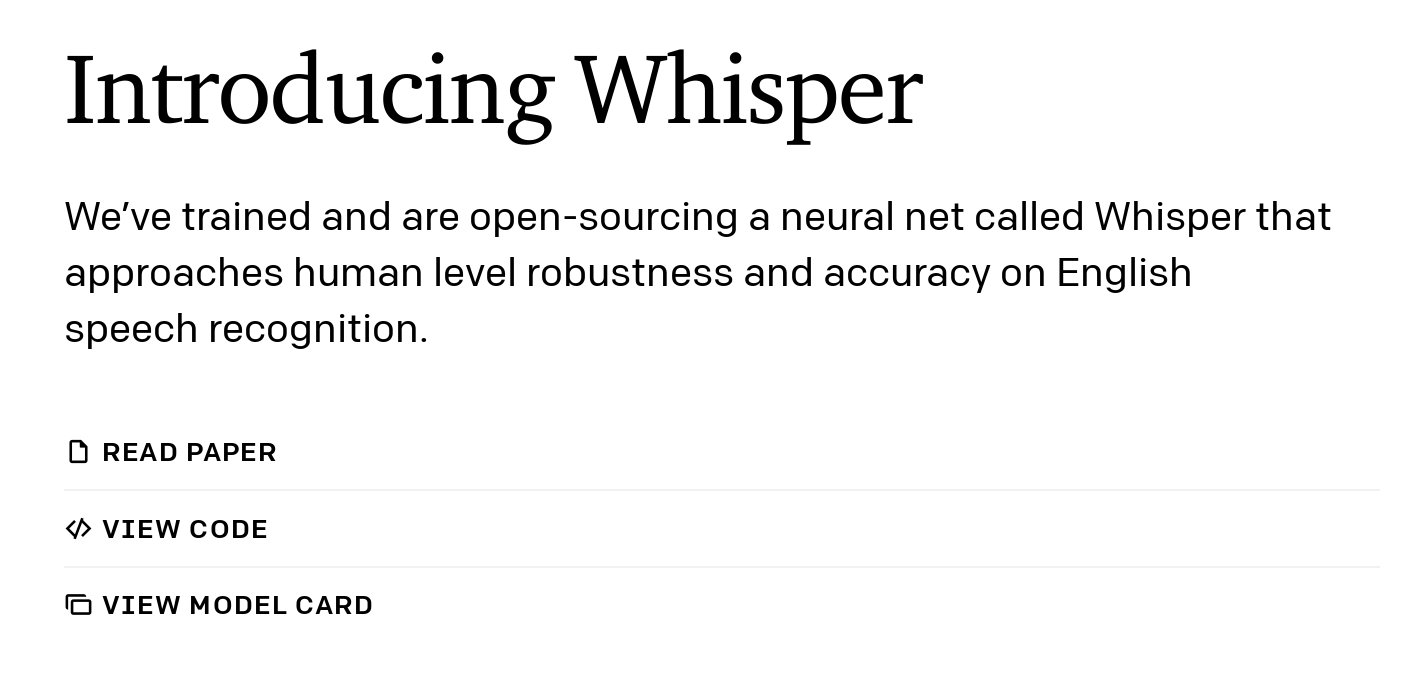
\includegraphics[width=8.5cm]{figs/whisper}

  \begin{flushright}
    {\scriptsize
    \url{https://openai.com/blog/whisper/}
    \url{https://github.com/openai/whisper} \\
    License: MIT (open source) \\
  }
  \end{flushright}

\end{frame}

%% -----------------------------------------
\begin{frame}[fragile]
  \frametitle{BLOOM}

  The World’s Largest Open Multilingual Language Model  

  176 billion parameters

  46 natural languages and 13 programming languages

  \begin{flushright}
    \url{https://bigscience.huggingface.co/blog/bloom} \\
    \url{https://huggingface.co/bigscience/bloom}
    License: BigScience RAIL License v1.0 (restricted use cases) \\
  \end{flushright}

\end{frame}

%% -----------------------------------------
\begin{frame}[fragile]
  \frametitle{Multilingual AI Assistant}

   Whisper for Speech-to-text  \\
   Bloom for Text-generation, \\
   CoquiTTS for Text-To-Speech \\
  
  \begin{flushright}
    {\scriptsize
      \url{https://huggingface.co/spaces/ysharma/Talk_to_Multilingual_AI_WhisperBloomCoqui} \\
    }
  \end{flushright}

\end{frame}

%% -----------------------------------------
\begin{frame}[fragile]
  \frametitle{Whisper to Stable Diffusion}

  
  \begin{flushright}
    {\scriptsize
      \url{https://huggingface.co/spaces/fffiloni/whisper-to-stable-diffusion} \\
    }
  \end{flushright}

\end{frame}

%%-----------------------------------------
\begin{frame}[fragile]
  \frametitle{Whisper for YouTube captions}

  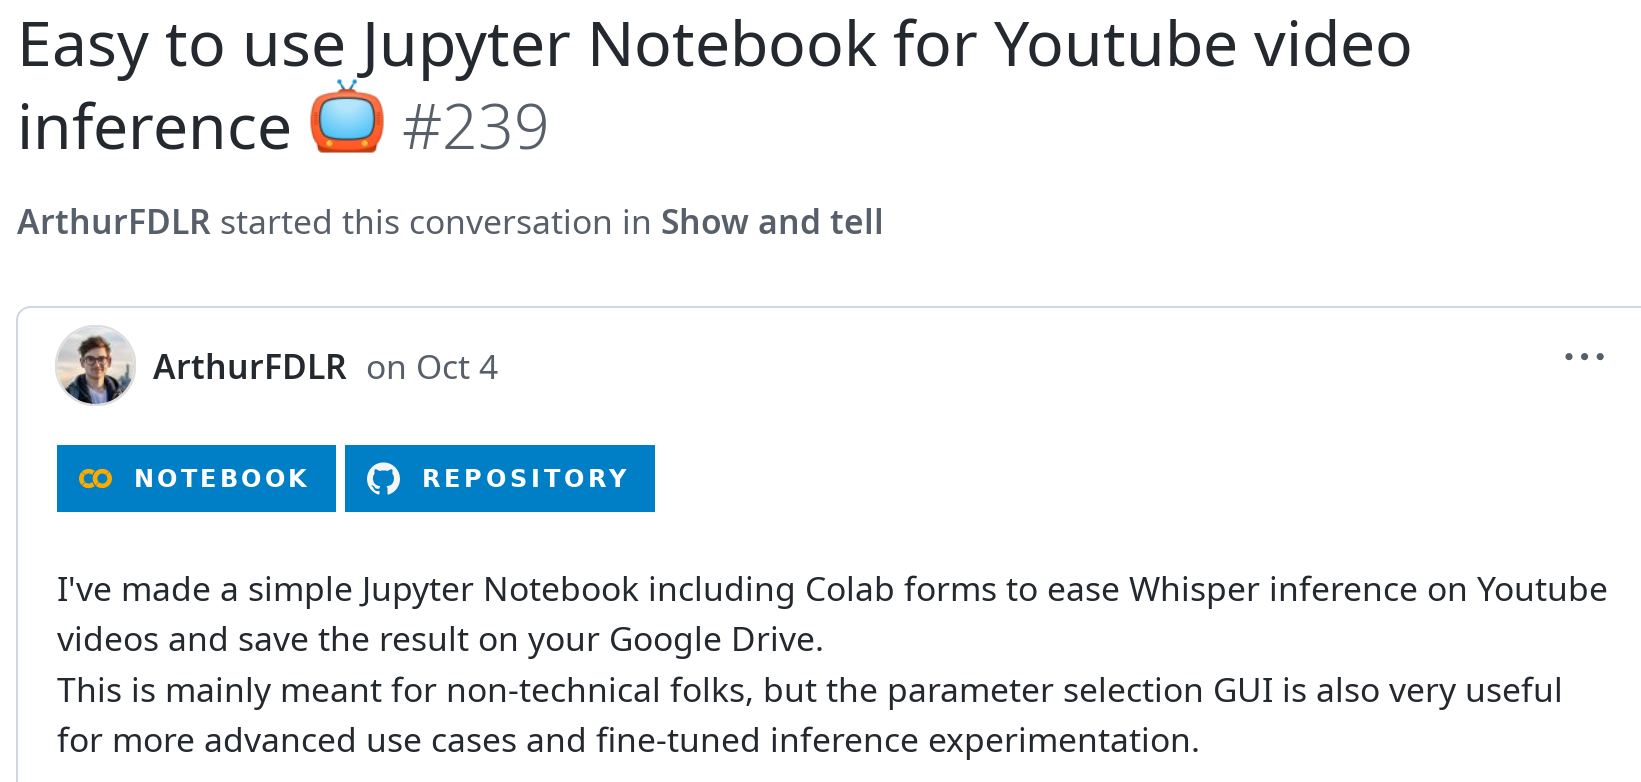
\includegraphics[width=8.5cm]{figs/whisper-youtube}

  \begin{flushright}
    {\scriptsize
    \url{https://github.com/openai/whisper/discussions/239}
  }
  \end{flushright}

\end{frame}


%%-----------------------------------------
\begin{frame}[fragile]
  \frametitle{Toonification of faces}

  From picture to toonified picture

  From video to toonified video
  
  \begin{flushright}
    \url{https://huggingface.co/spaces/PKUWilliamYang/VToonify} \\
    \url{https://github.com/williamyang1991/VToonify} \\
    License: S-Lab License 1.0 (non-commercial) \\
  \end{flushright}

\end{frame}

%%-----------------------------------------
\begin{frame}[fragile]
  \frametitle{Musika}

  Fast 44.1 kHz stereo waveform music generation of arbitrary length

  \begin{flushright}
    \url{https://arxiv.org/abs/2208.08706} \\
    \url{https://huggingface.co/spaces/marcop/musika} \\
    License: MIT (open source) \\
  \end{flushright}

\end{frame}

%%-----------------------------------------
\begin{frame}[fragile]
  \frametitle{Queries to documents}

  \begin{columns}[T]
    \begin{column}{.58\textwidth}
      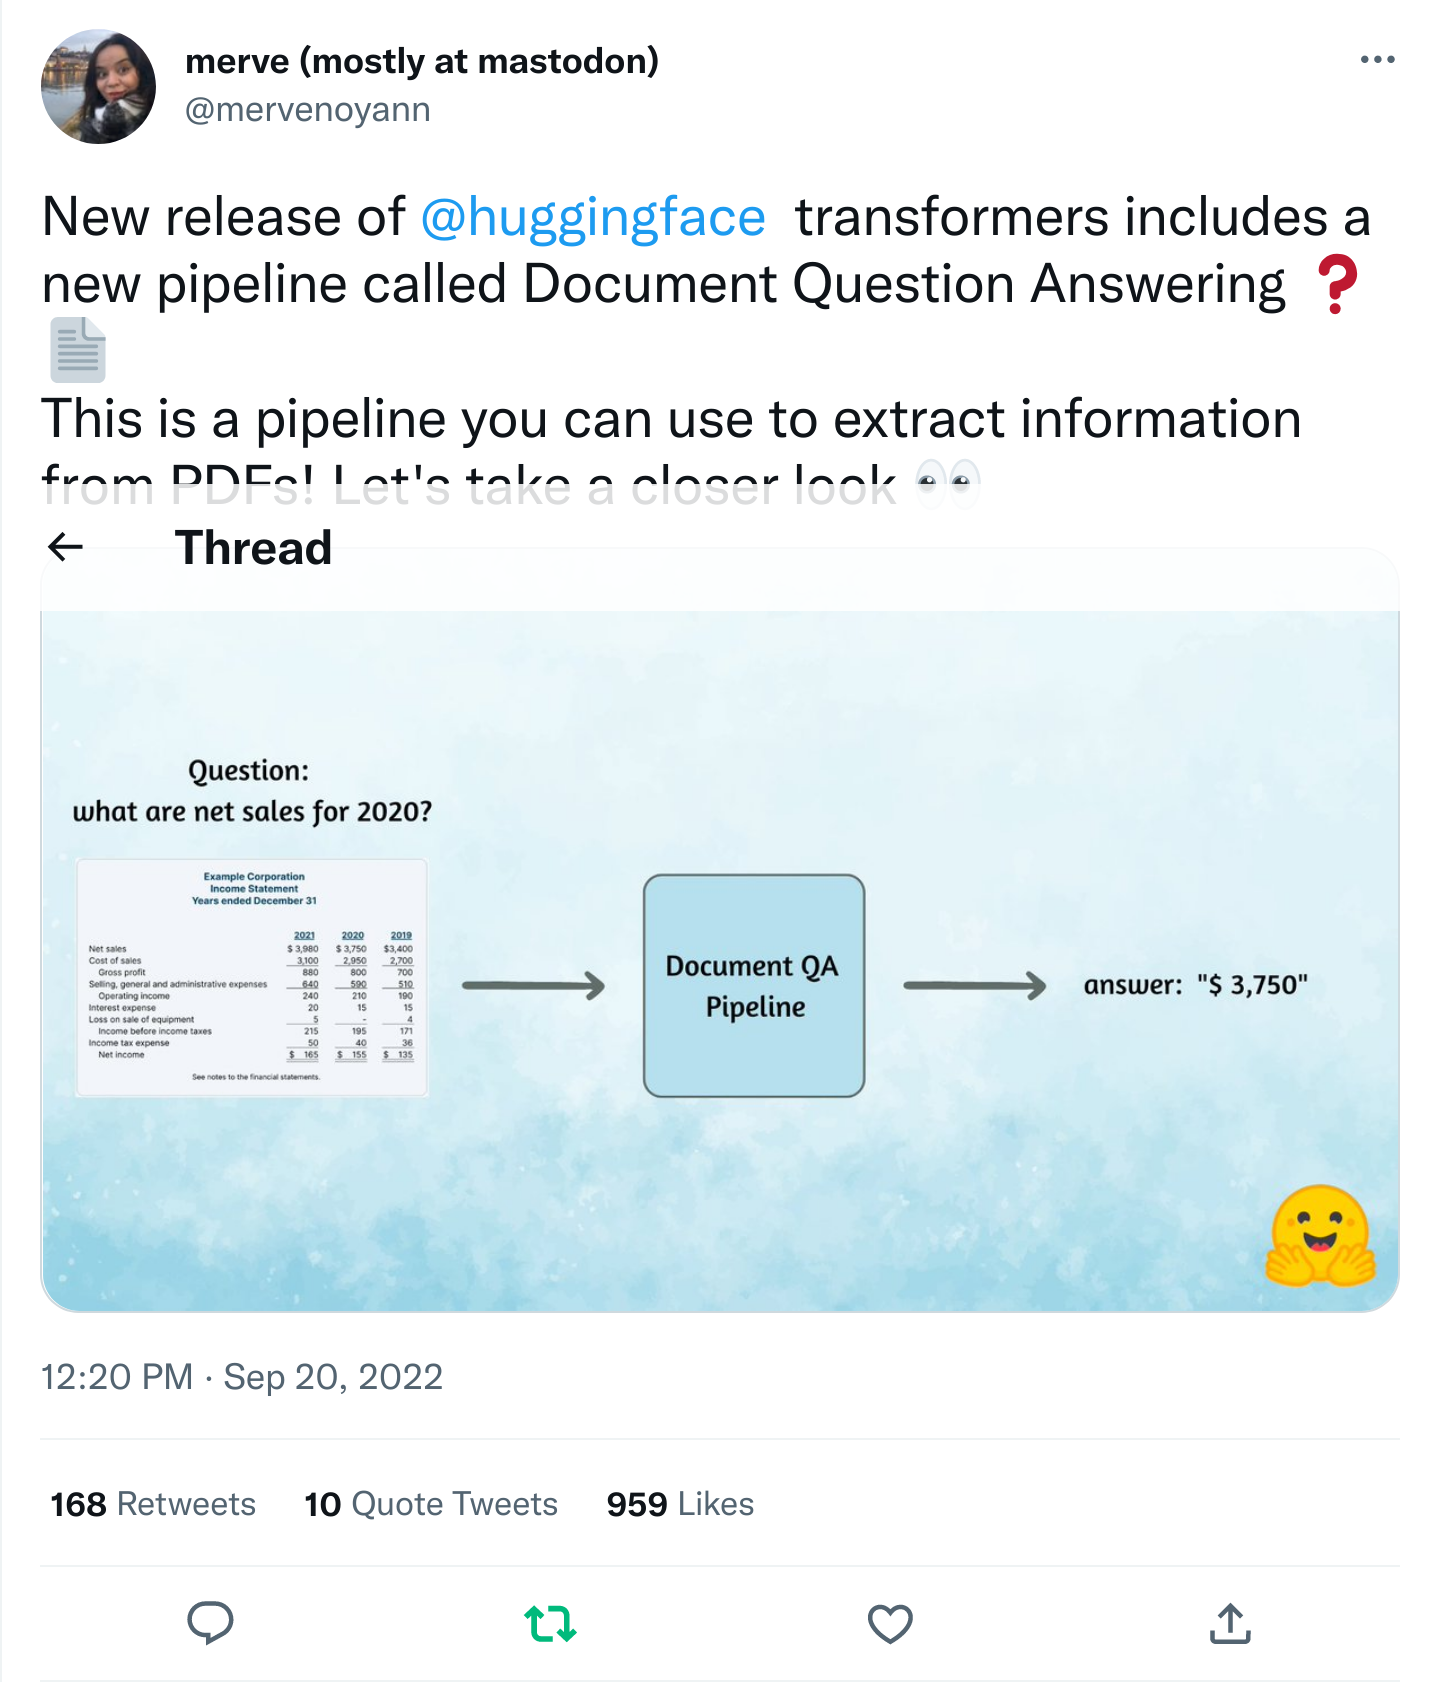
\includegraphics[width=7.5cm]{figs/pdf-extract}
    \end{column}%
    \hfill%
    \begin{column}{.38\textwidth}
      \vspace{1.5cm}
    {\scriptsize
      \url{https://twitter.com/mervenoyann/status/1572168848622907393}
    }
    \end{column}%
  \end{columns}

\end{frame}

%%-----------------------------------------
%%-----------------------------------------
\section{Infrastructure to play, to share}


%%-----------------------------------------
\begin{frame}[fragile]
  \frametitle{Hugging Face}

  \begin{columns}[T]
    \begin{column}{.58\textwidth}
        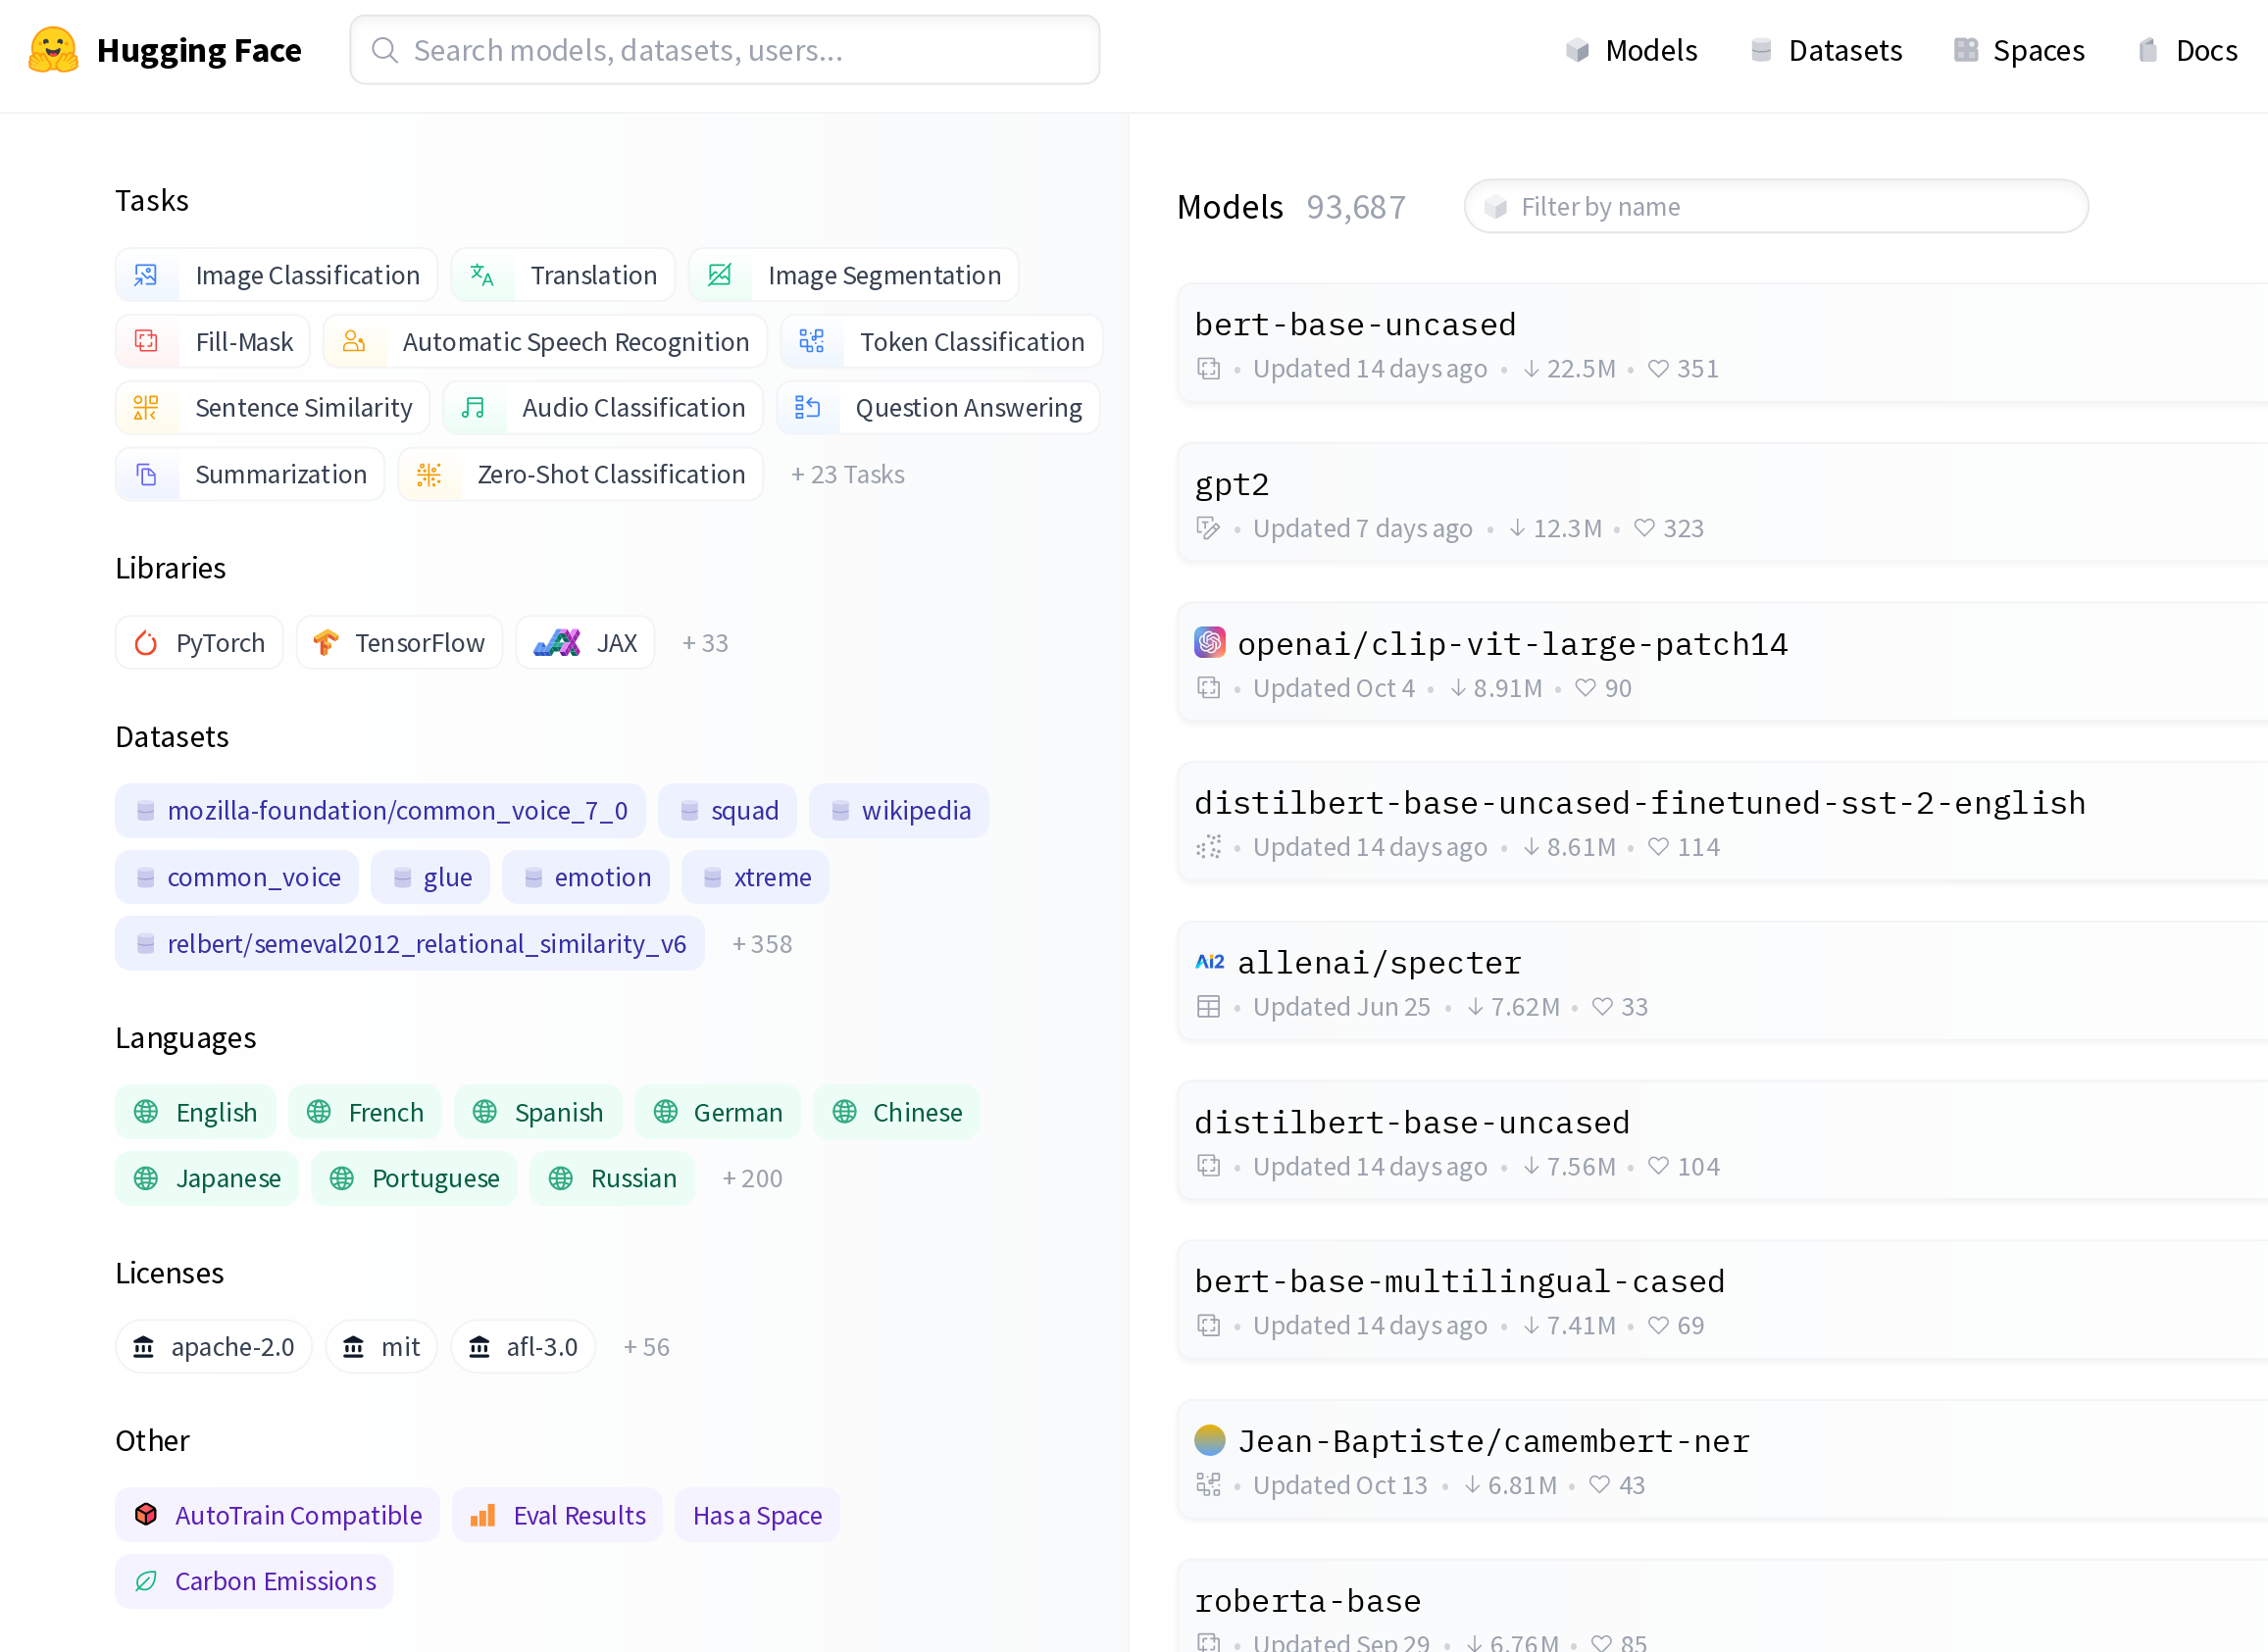
\includegraphics[width=7.5cm]{figs/hugging-face}
    \end{column}%
    \hfill%
    \begin{column}{.38\textwidth}
        ``GitHub for ML''

        \vspace{2cm}
        
        {\scriptsize
          \url{https://huggingface.co} \\
        }
    \end{column}%
  \end{columns}

\end{frame}

%%-----------------------------------------
\begin{frame}[fragile]
  \frametitle{Gradio}

  \begin{center}
    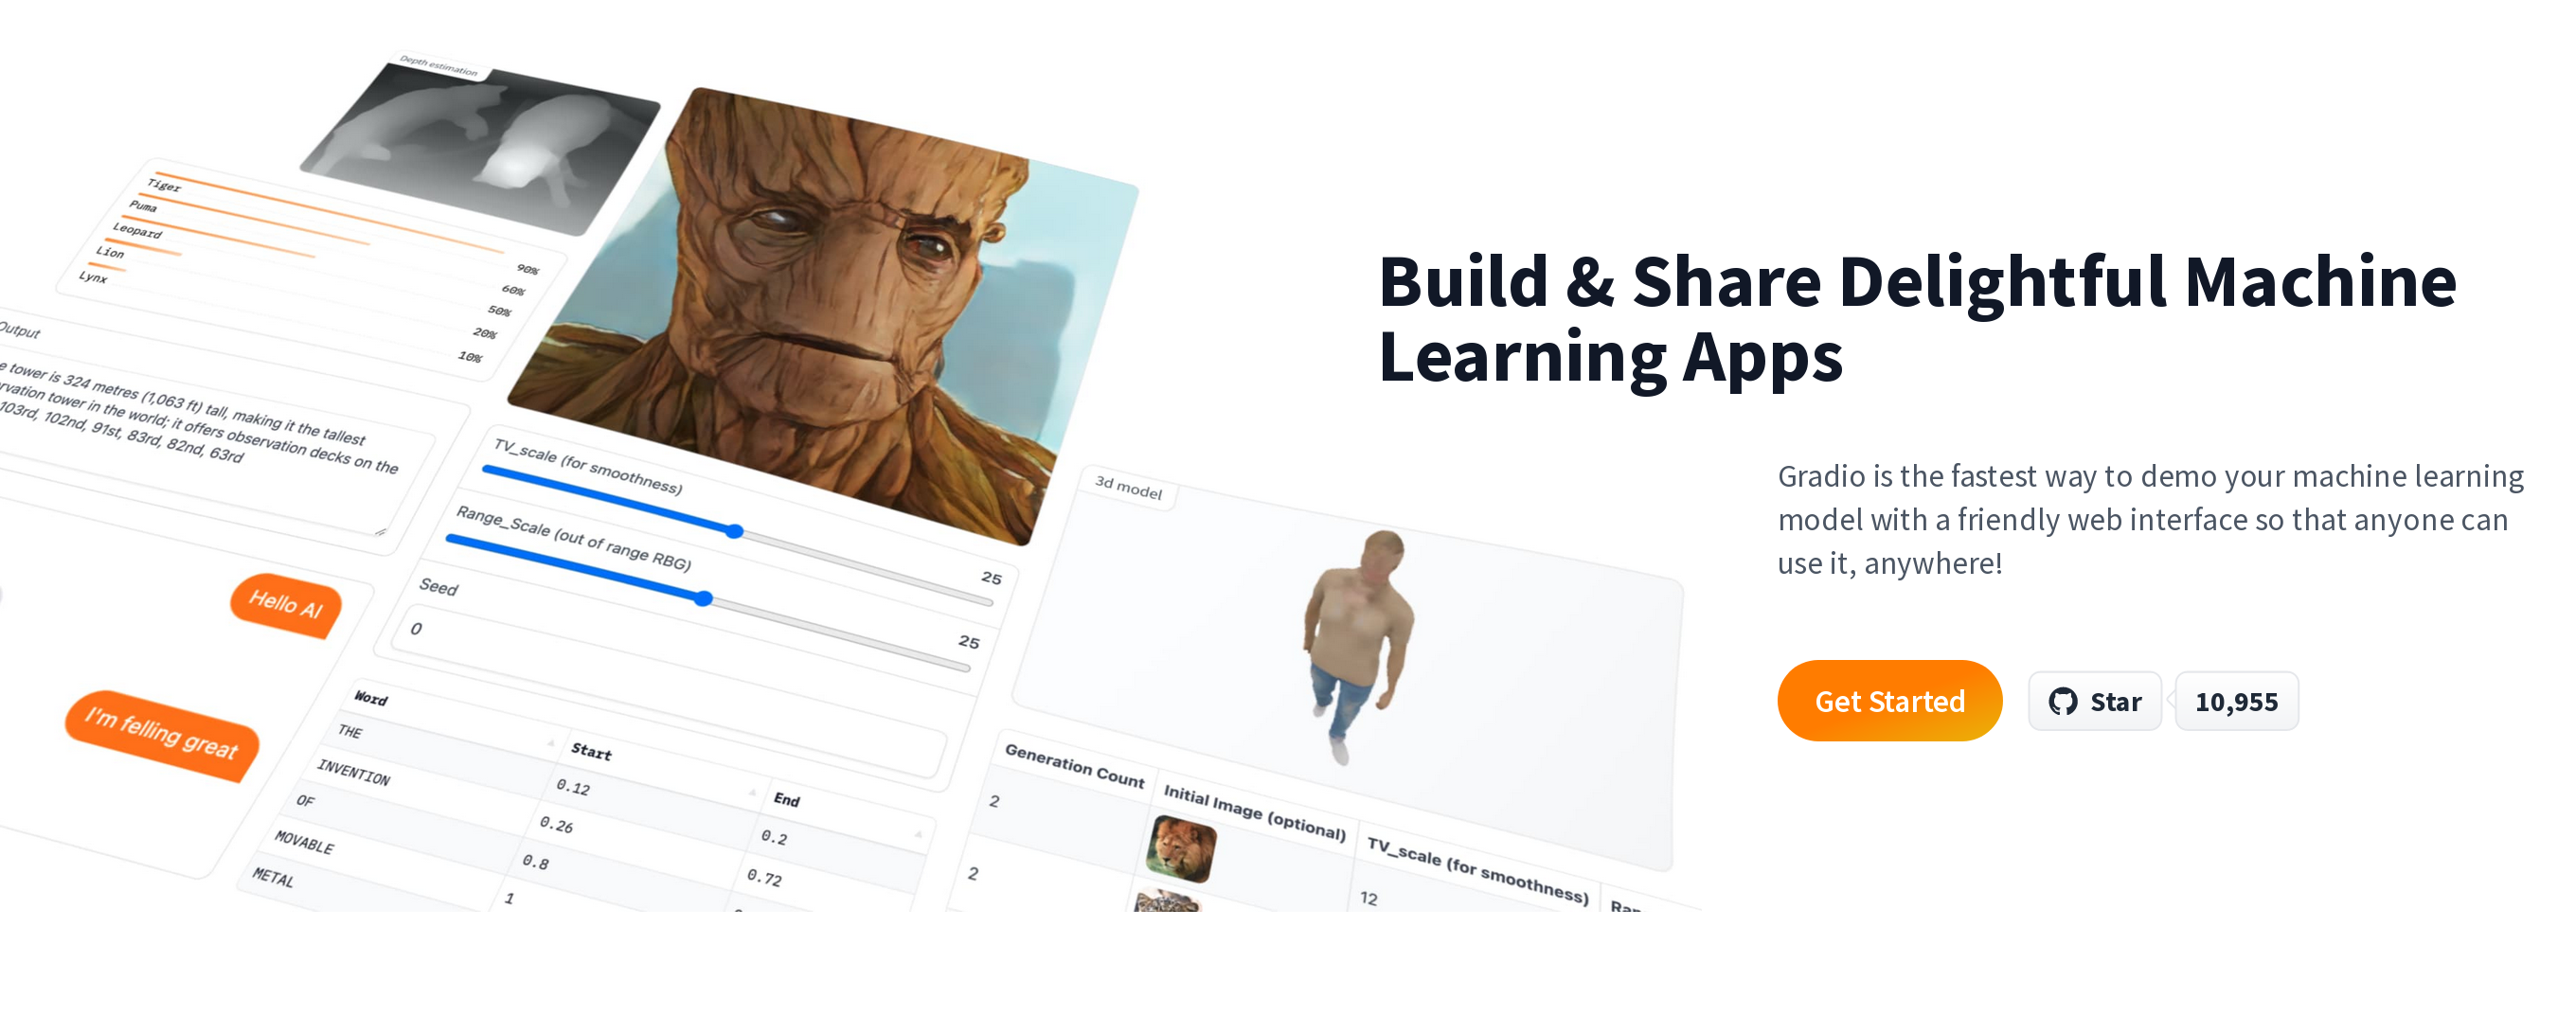
\includegraphics[width=12cm]{figs/gradio}
  \end{center}

  \begin{flushright}
    {\small
      \url{https://gradio.app/} \\
      License: Apache 2.0 \\
    }
  \end{flushright}
\end{frame}

%%-----------------------------------------
\begin{frame}[fragile]
  \frametitle{Diffusers}

  \begin{center}
    
\includegraphics[width=8cm]{figs/diffusers}
  \end{center}

  Pretrained diffusion models (vision, audio, etc.) \\
  Modular toolbox for inference \& training of diffusion models \\


  \begin{flushright}
    {\small
      \url{https://github.com/huggingface/diffusers} \\
      License: Apache 2.0 \\
    }
  \end{flushright}
\end{frame}

%%-----------------------------------------
\begin{frame}[fragile]
  \frametitle{Model frameworks, etc}

    \begin{columns}[T]
    \begin{column}{.28\textwidth}

  \begin{flushright}
        PyTorch
  \end{flushright}

  \begin{flushright}
        TensorFlow
  \end{flushright}

  \begin{flushright}
        Keras
  \end{flushright}

  \begin{flushright}
        Cuda
  \end{flushright}
    \end{column}%
    \hfill%
    \begin{column}{.68\textwidth}
  \begin{flushright}
    {\small \url{https://pytorch.org/}}
  \end{flushright}

   \begin{flushright}
    {\small  \url{https://tensorflow.org/}}
  \end{flushright}

  \begin{flushright}
    {\small  \url{https://keras.io/}}
  \end{flushright}

    \begin{flushright}
    {\small  \url{https://developer.nvidia.com/cuda-toolkit}}
  \end{flushright}
   \end{column}%
  \end{columns}

  
\end{frame}

%%-----------------------------------------
\begin{frame}[fragile]
  \frametitle{Collab}

  \begin{center}
    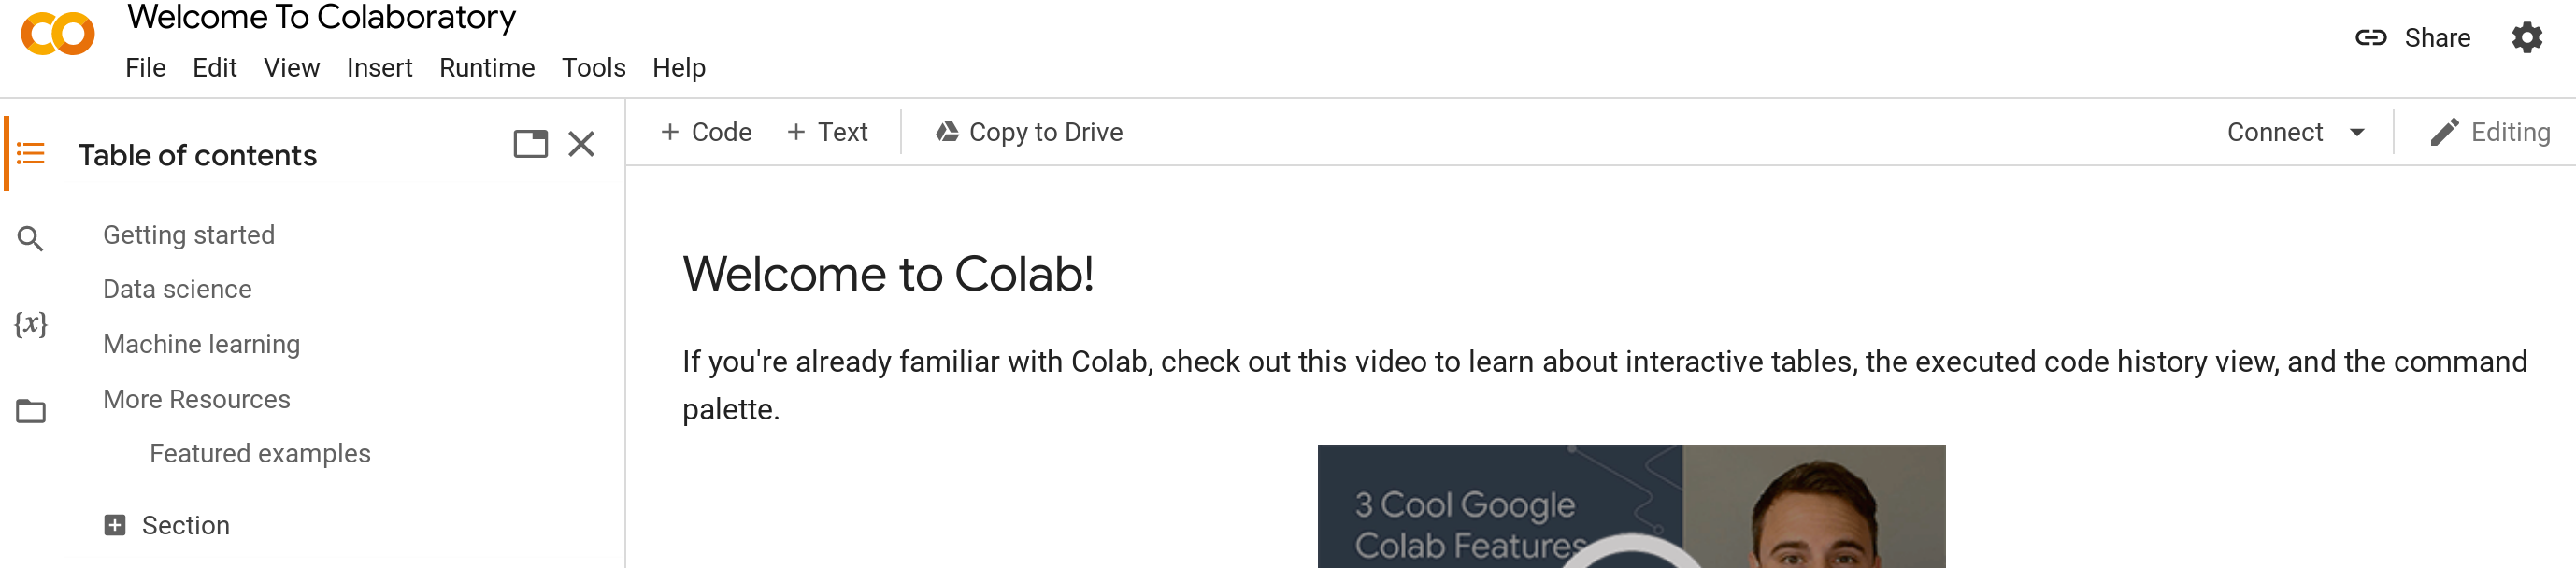
\includegraphics[width=12cm]{figs/collab}
  \end{center}

  Python in the browser, zero configuration \\
  Access to GPUs \& easy sharing \\

  \begin{flushright}
    {\small
      \url{https://colab.research.google.com/}
    }
  \end{flushright}
\end{frame}

%%-----------------------------------------
\begin{frame}[fragile]
  \frametitle{Jupyter}

  \begin{center}
    
\includegraphics[width=10cm]{figs/jupyter}
  \end{center}

  Python in the browser, easy

  \begin{flushright}
    {\small
      \url{https://jupyter.org/}
    }
  \end{flushright}
\end{frame}


%%-----------------------------------------
%%-----------------------------------------
\section{Many issues raised}


%%-----------------------------------------
\begin{frame}[fragile]
  \frametitle{Intellectual property (training set)}

  \begin{columns}[T]
    \begin{column}{.58\textwidth}
        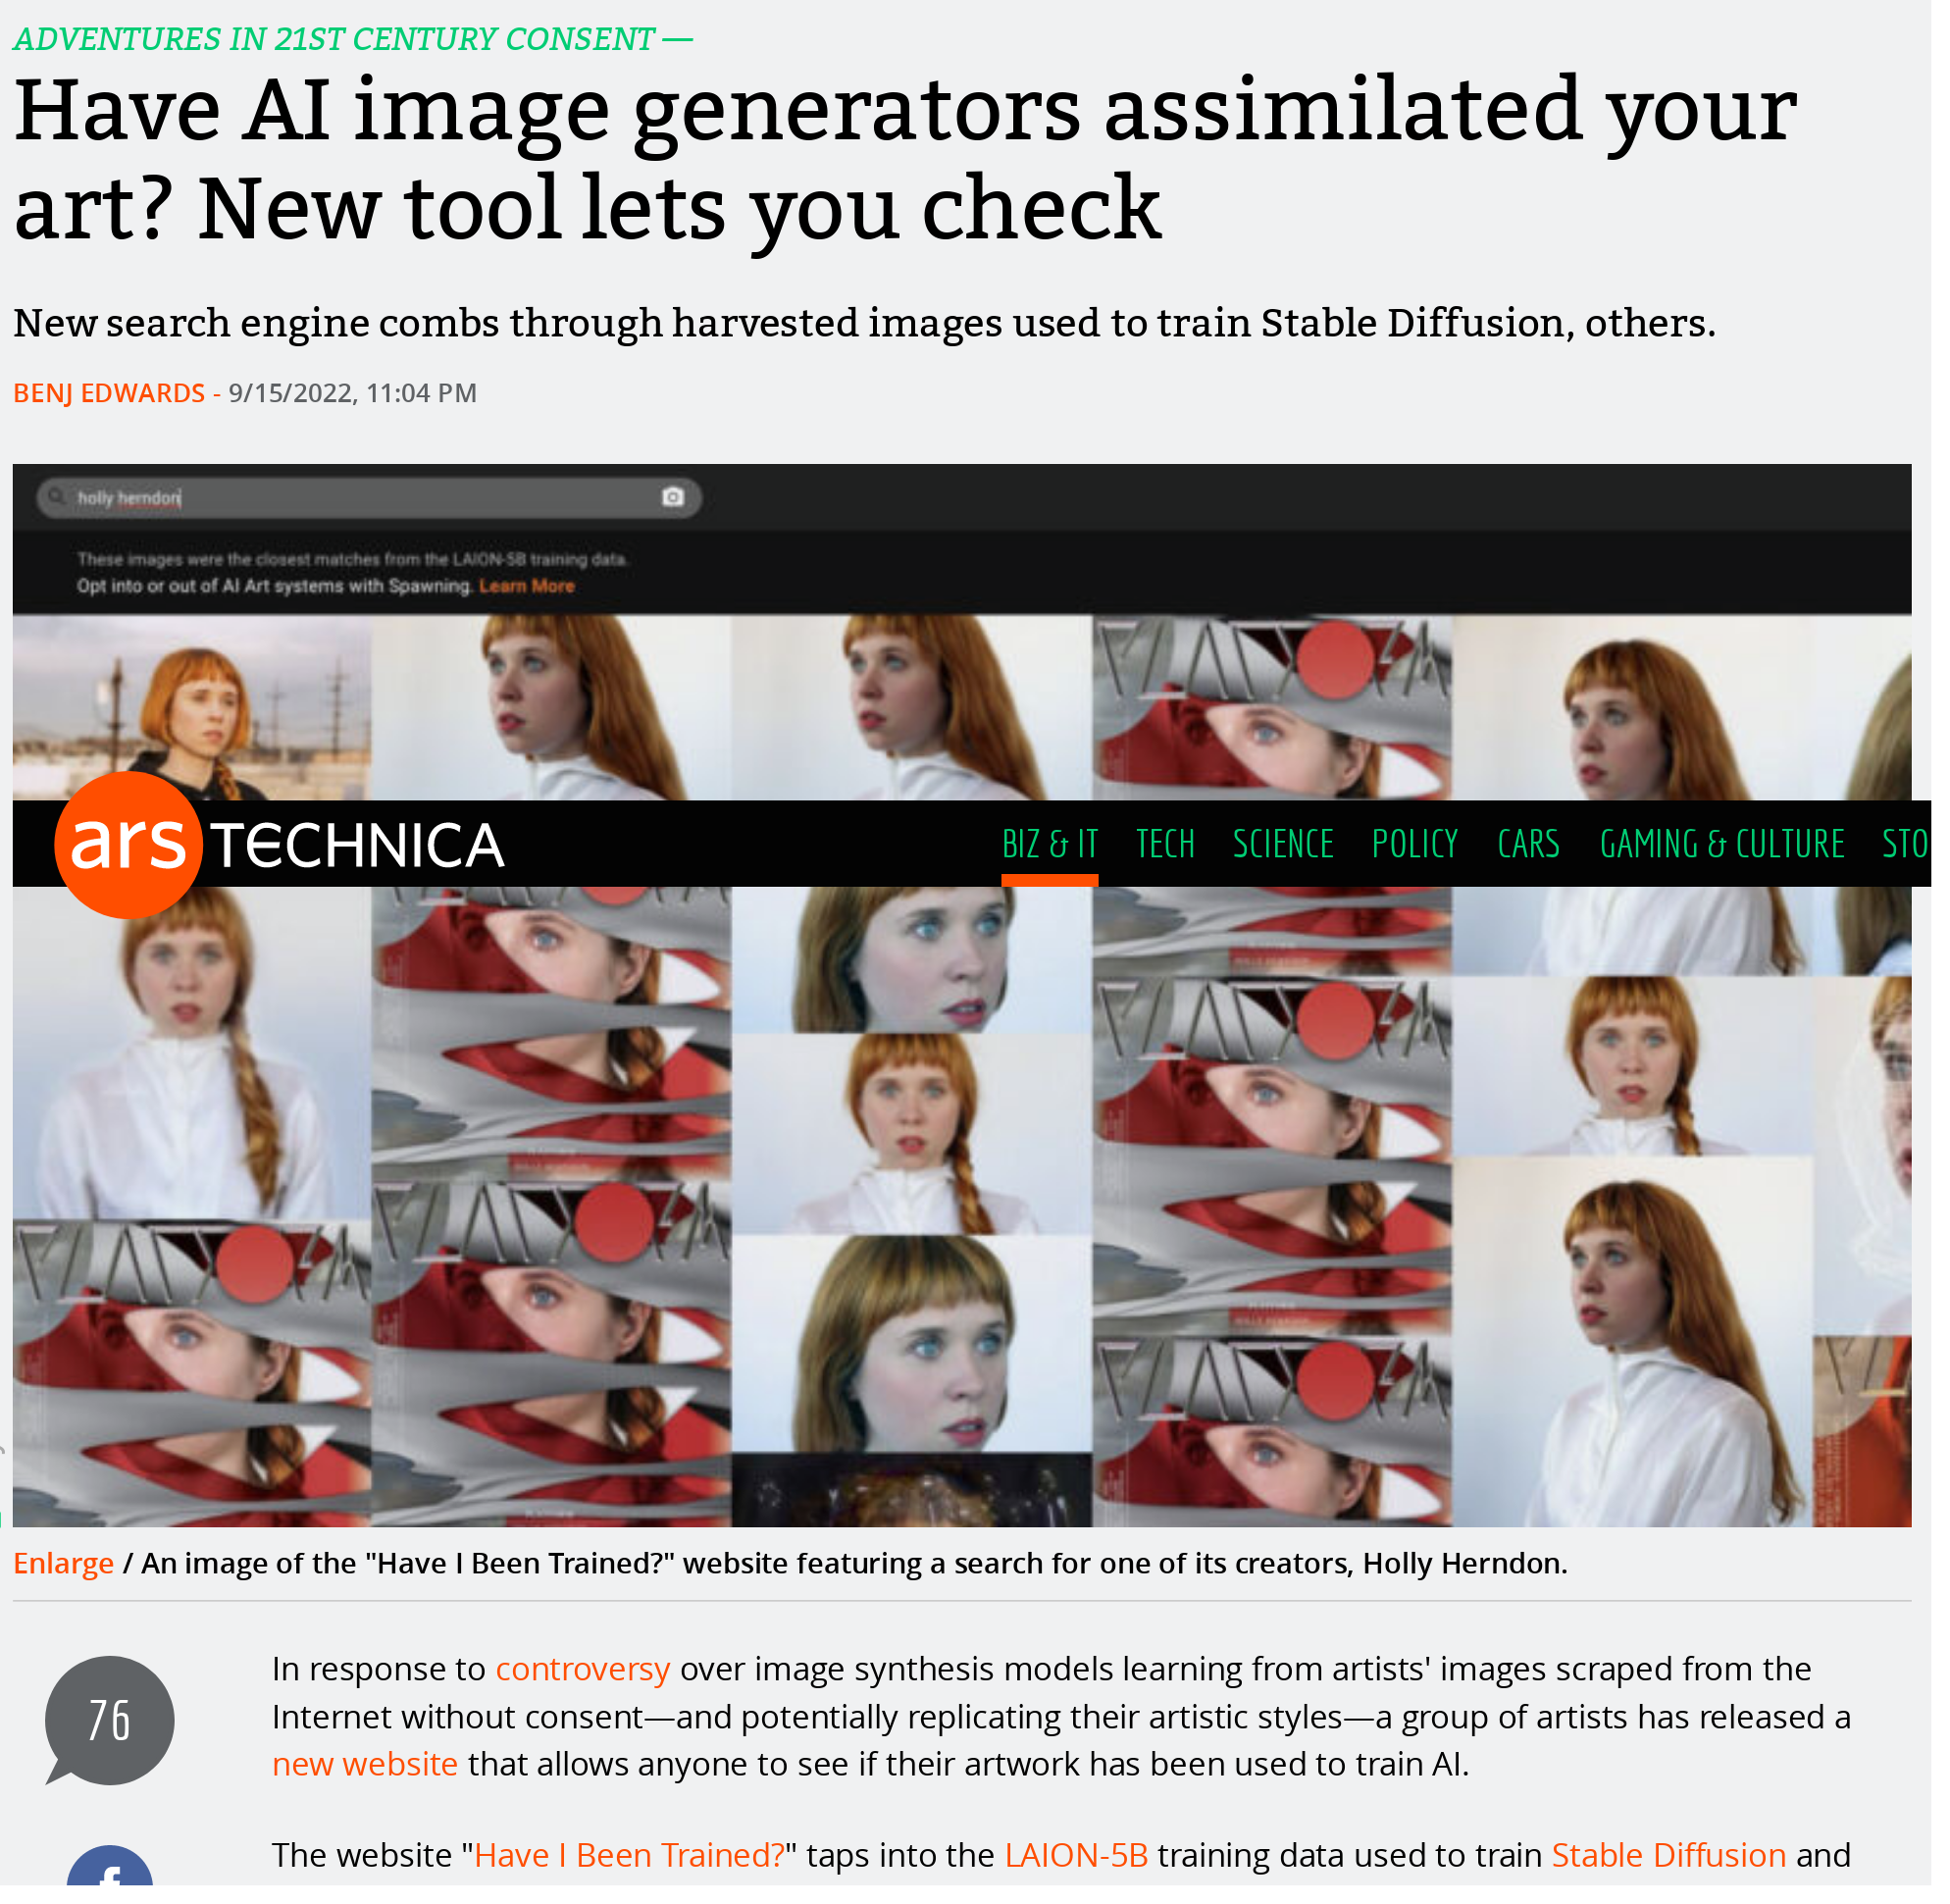
\includegraphics[width=7.5cm]{figs/used-art}
    \end{column}%
    \hfill%
    \begin{column}{.38\textwidth}

        \vspace{0.5cm}
        
        {\scriptsize
          \url{https://haveibeentrained.com/} \\

          \vspace{1cm}
      
          \url{https://arstechnica.com/information-technology/2022/09/have-ai-image-generators-assimilated-your-art-new-tool-lets-you-check/} \\
        }
    \end{column}%
  \end{columns}
  
\end{frame}


%%-----------------------------------------
\begin{frame}[fragile]
  \frametitle{Intellectual property (results)}

        
\includegraphics[width=7.5cm]{figs/impact-ai-copyright}
  
        {\scriptsize
          \url{https://euipo.europa.eu/tunnel-web/secure/webdav/guest/document_library/observatory/documents/reports/2022_Impact_AI_on_the_Infringement_and_Enforcement_CR_Designs/2022_Impact_AI_on_the_Infringement_and_Enforcement_CR_Designs_FullR_en.pdf} \\
        }
        
\end{frame}

%%-----------------------------------------
\begin{frame}[fragile]
  \frametitle{Intellectual property}

  \begin{itemize}
  \item Can models be trained on anything public?

  \item Are models subject to copyright law?

  \item Who is the author of the production of a model?

  \item Can anybody besides the author claim rights on the production of a model
  \end{itemize}
  
\end{frame}

%%-----------------------------------------
\begin{frame}[fragile]
  \frametitle{Licenses}

  \begin{columns}[T]
    \begin{column}{.36\textwidth}
        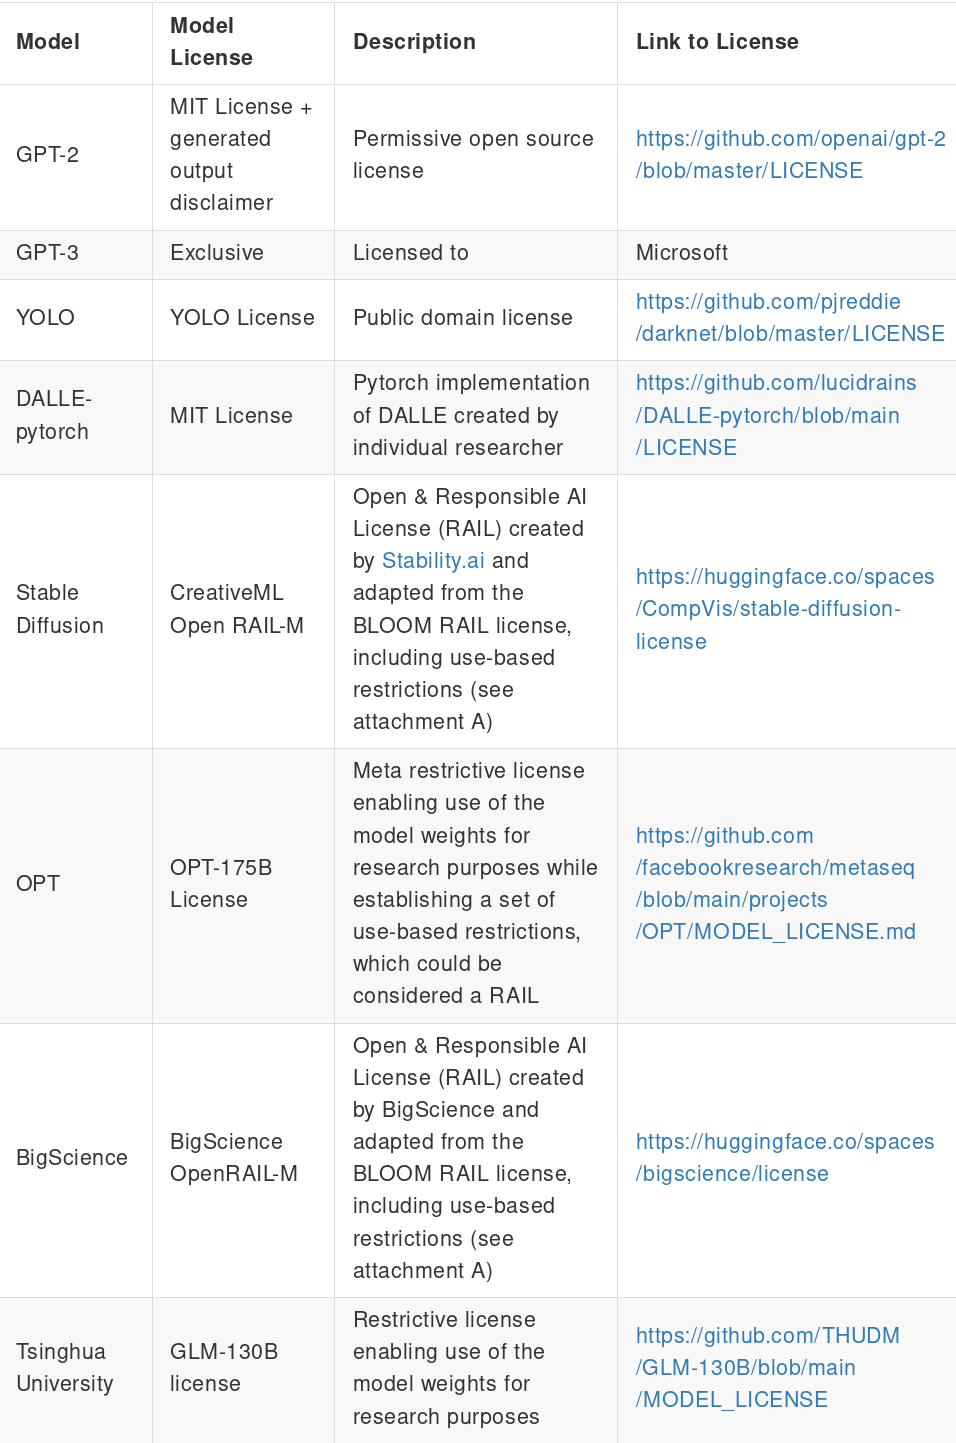
\includegraphics[width=4cm]{figs/licensing}
    \end{column}%
    \hfill%
    \begin{column}{.62\textwidth}

        \vspace{0.5cm}
        
        {\scriptsize
          \url{https://hackmd.io/@jending12/HyvMU8sJo} \\

          \vspace{1.5cm}
          \url{https://thegradient.pub/machine-learning-ethics-and-open-source-licensing-2/}
        }
    \end{column}%
  \end{columns}
  
\end{frame}

%%-----------------------------------------
\begin{frame}[fragile]
  \frametitle{Bias}

    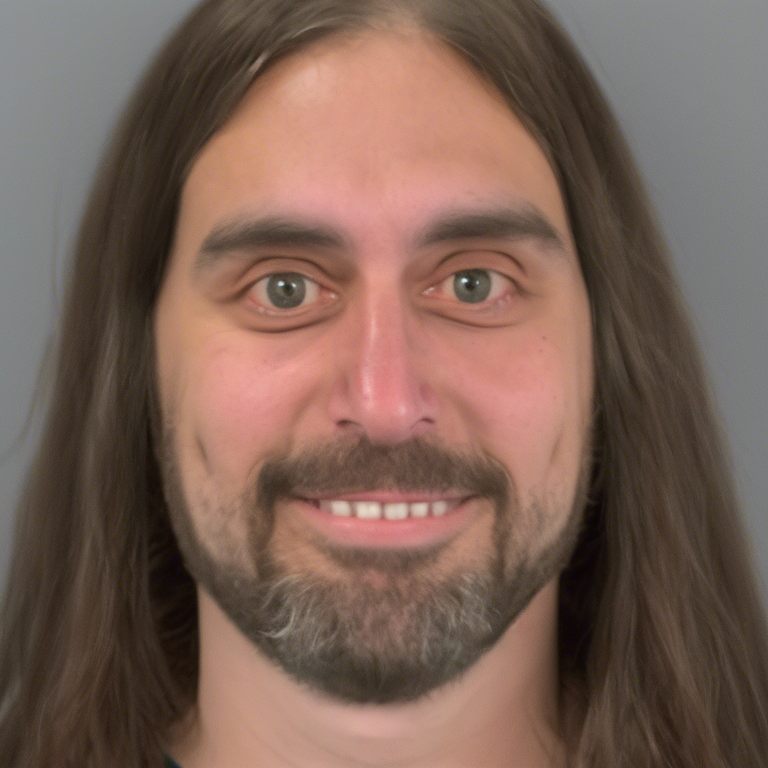
\includegraphics[width=2cm]{figs/17a}
    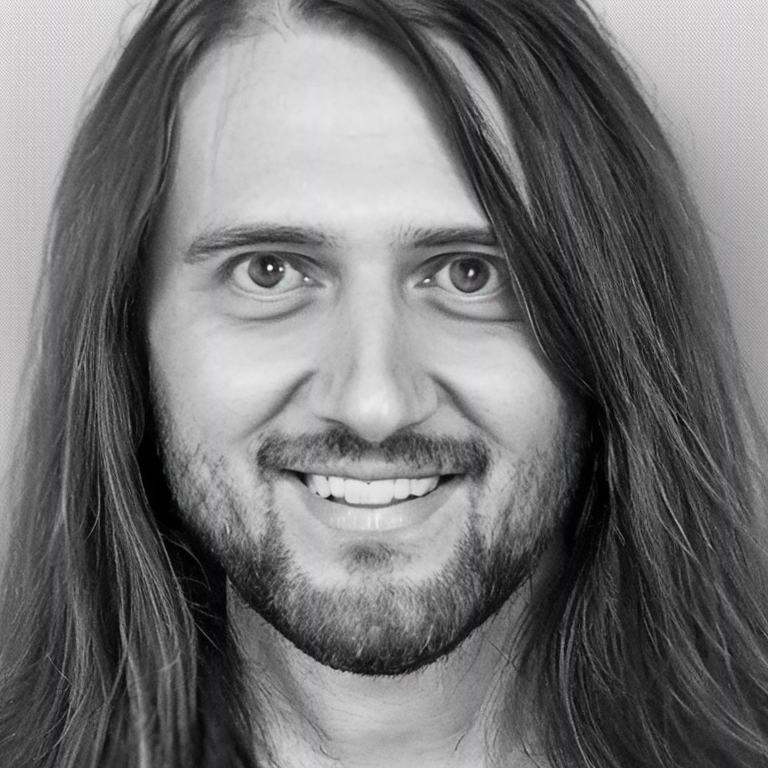
\includegraphics[width=2cm]{figs/17b}
    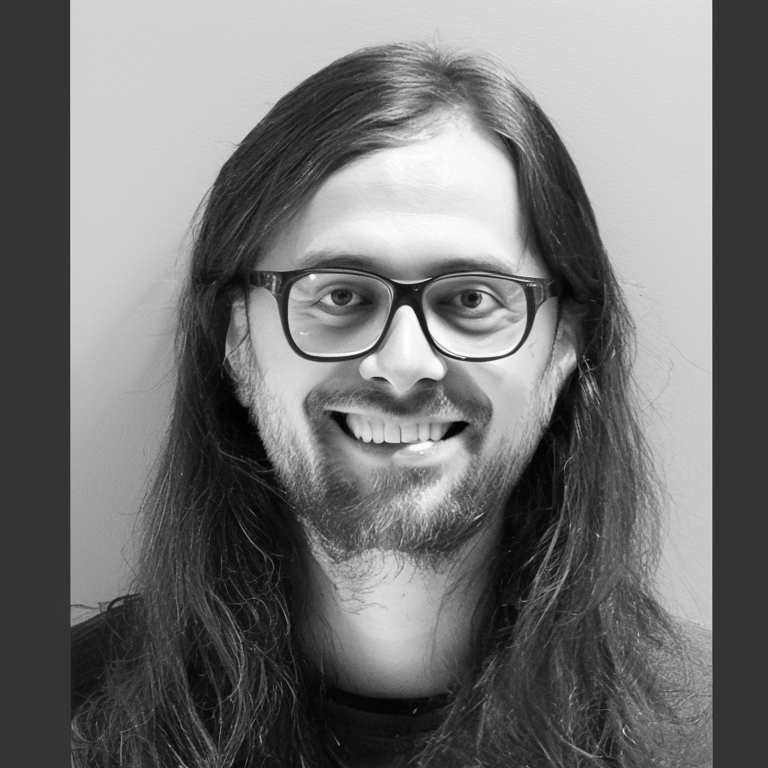
\includegraphics[width=2cm]{figs/17c}
    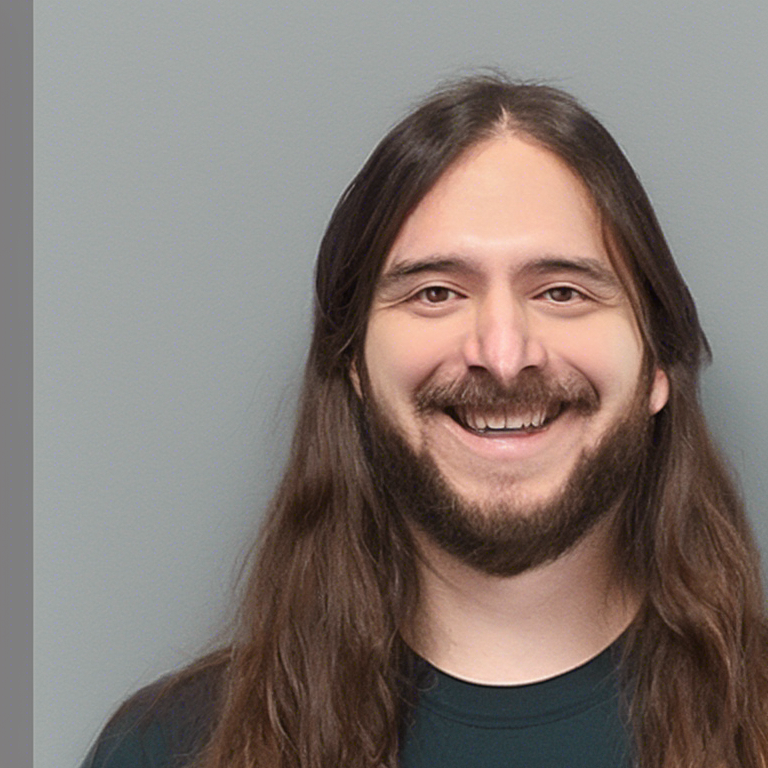
\includegraphics[width=2cm]{figs/17d}
  
    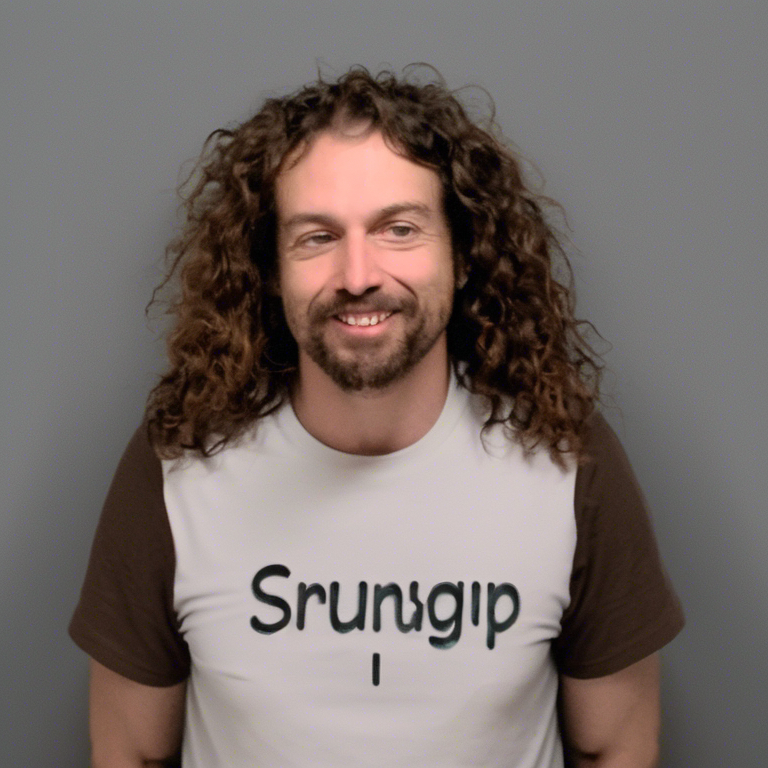
\includegraphics[width=2cm]{figs/18a}
    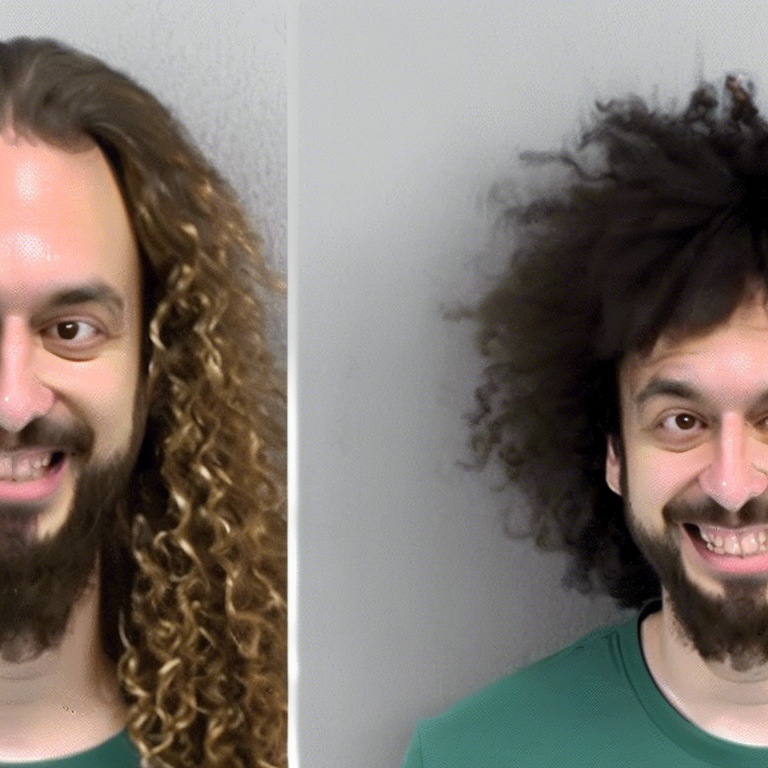
\includegraphics[width=2cm]{figs/18b}
    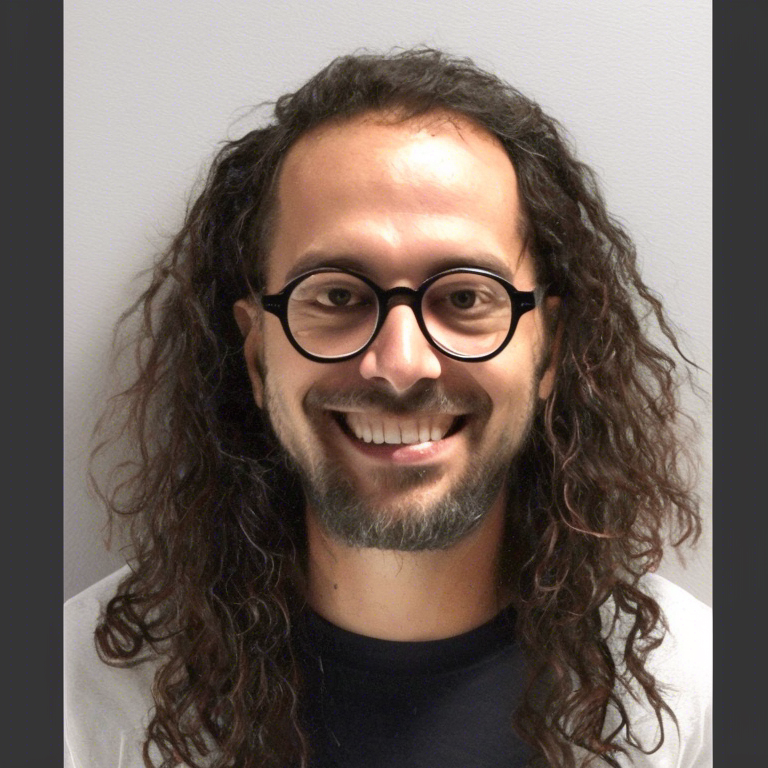
\includegraphics[width=2cm]{figs/18c}
    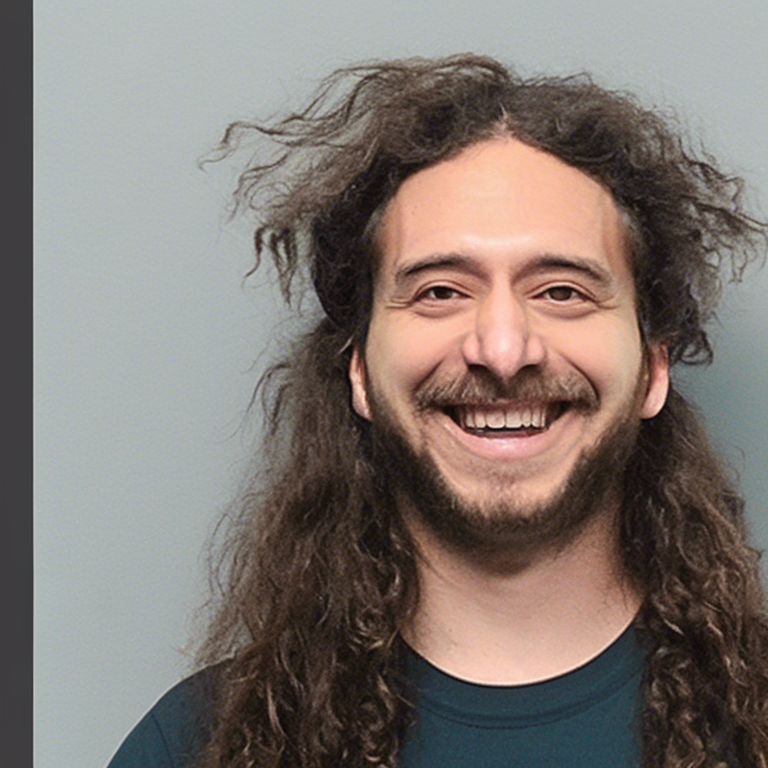
\includegraphics[width=2cm]{figs/18d}

    {\small
      Mugshot of a technical speaker, machine learning expert, smiling, long hair, big eyes [t-shirt, curly hair]
    }

\end{frame}

%%-----------------------------------------
\begin{frame}[fragile]
  \frametitle{Security}

  
\includegraphics[width=9cm]{figs/ml-attacks}

  {\scriptsize
    \url{https://research.nccgroup.com/2022/07/06/whitepaper-practical-attacks-on-machine-learning-systems/} \\
    \url{https://simonwillison.net/2022/Sep/12/prompt-injection/} \\
    }
  
\end{frame}

%%-----------------------------------------
\begin{frame}[fragile]
  \frametitle{Impact on professionals}

  \begin{itemize}
  \item No more draw for hire as a profession?
  \item New opportunities for artists?
  \item Access to models as a fundamental need?
  \end{itemize}

  
  Is this different from the invention of photography?
\end{frame}

%%-----------------------------------------
\begin{frame}[fragile]
  \frametitle{Impact on professionals}

  {\Large
  Is this different \\
  from the invention of photography? \\
}

\end{frame}

%%-----------------------------------------
\begin{frame}[fragile]
  \frametitle{Prompt engineers}

  A new profession

  \vspace{.5cm}

  Artists, engineers, craftsmen?

  \vspace{.5cm}

  Is it here to stay?
  
\end{frame}

%%-----------------------------------------
\begin{frame}[fragile]
  \frametitle{What is true?}

    \begin{center}
    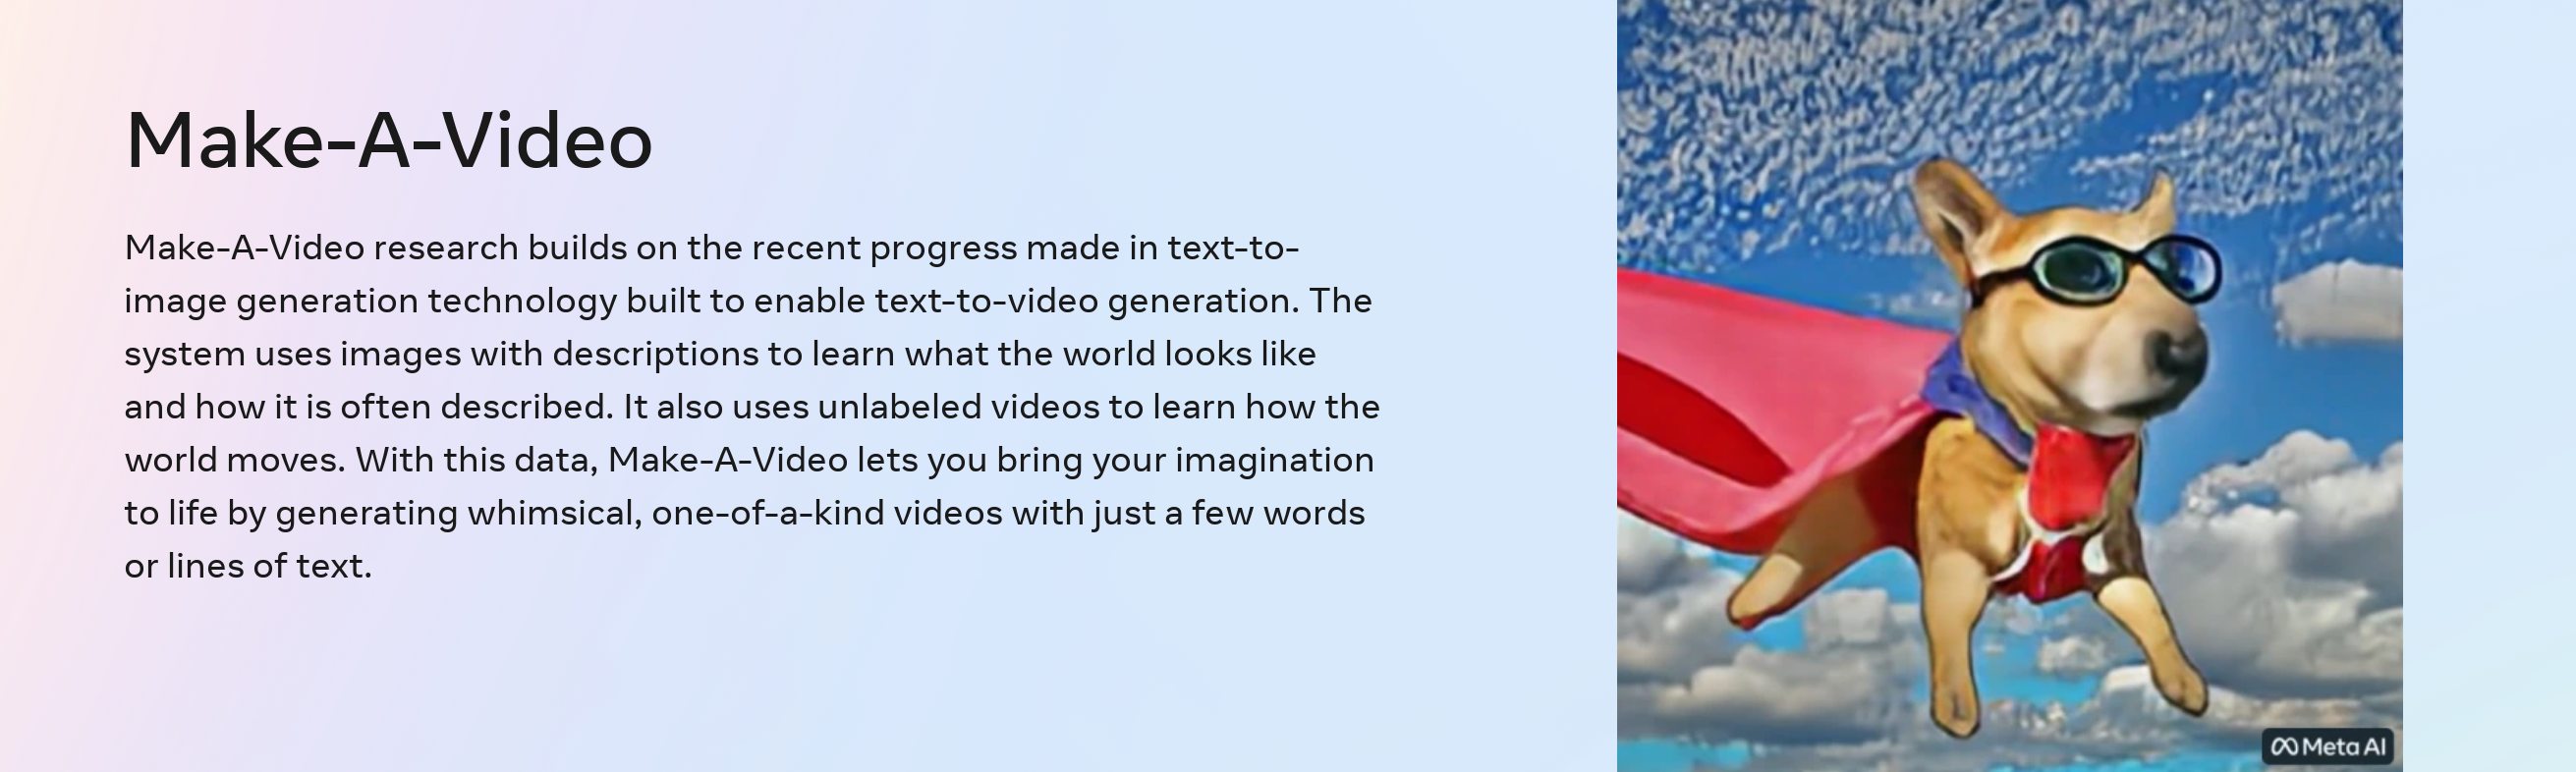
\includegraphics[width=9.5cm]{figs/makeavideo}
  \end{center}
  
  \begin{flushright}
    {\scriptsize
      \url{https://makeavideo.studio/}
    }
  \end{flushright}

  
\end{frame}


%%-----------------------------------------
%%-----------------------------------------
\section{The future}

%%-----------------------------------------
\begin{frame}[fragile]
  \frametitle{Assignments}

  \begin{center}
    
\includegraphics[width=7cm]{figs/kids-essays}
  \end{center}

  
\end{frame}

%%-----------------------------------------
\begin{frame}[fragile]
  \frametitle{Programming}

  \begin{center}
    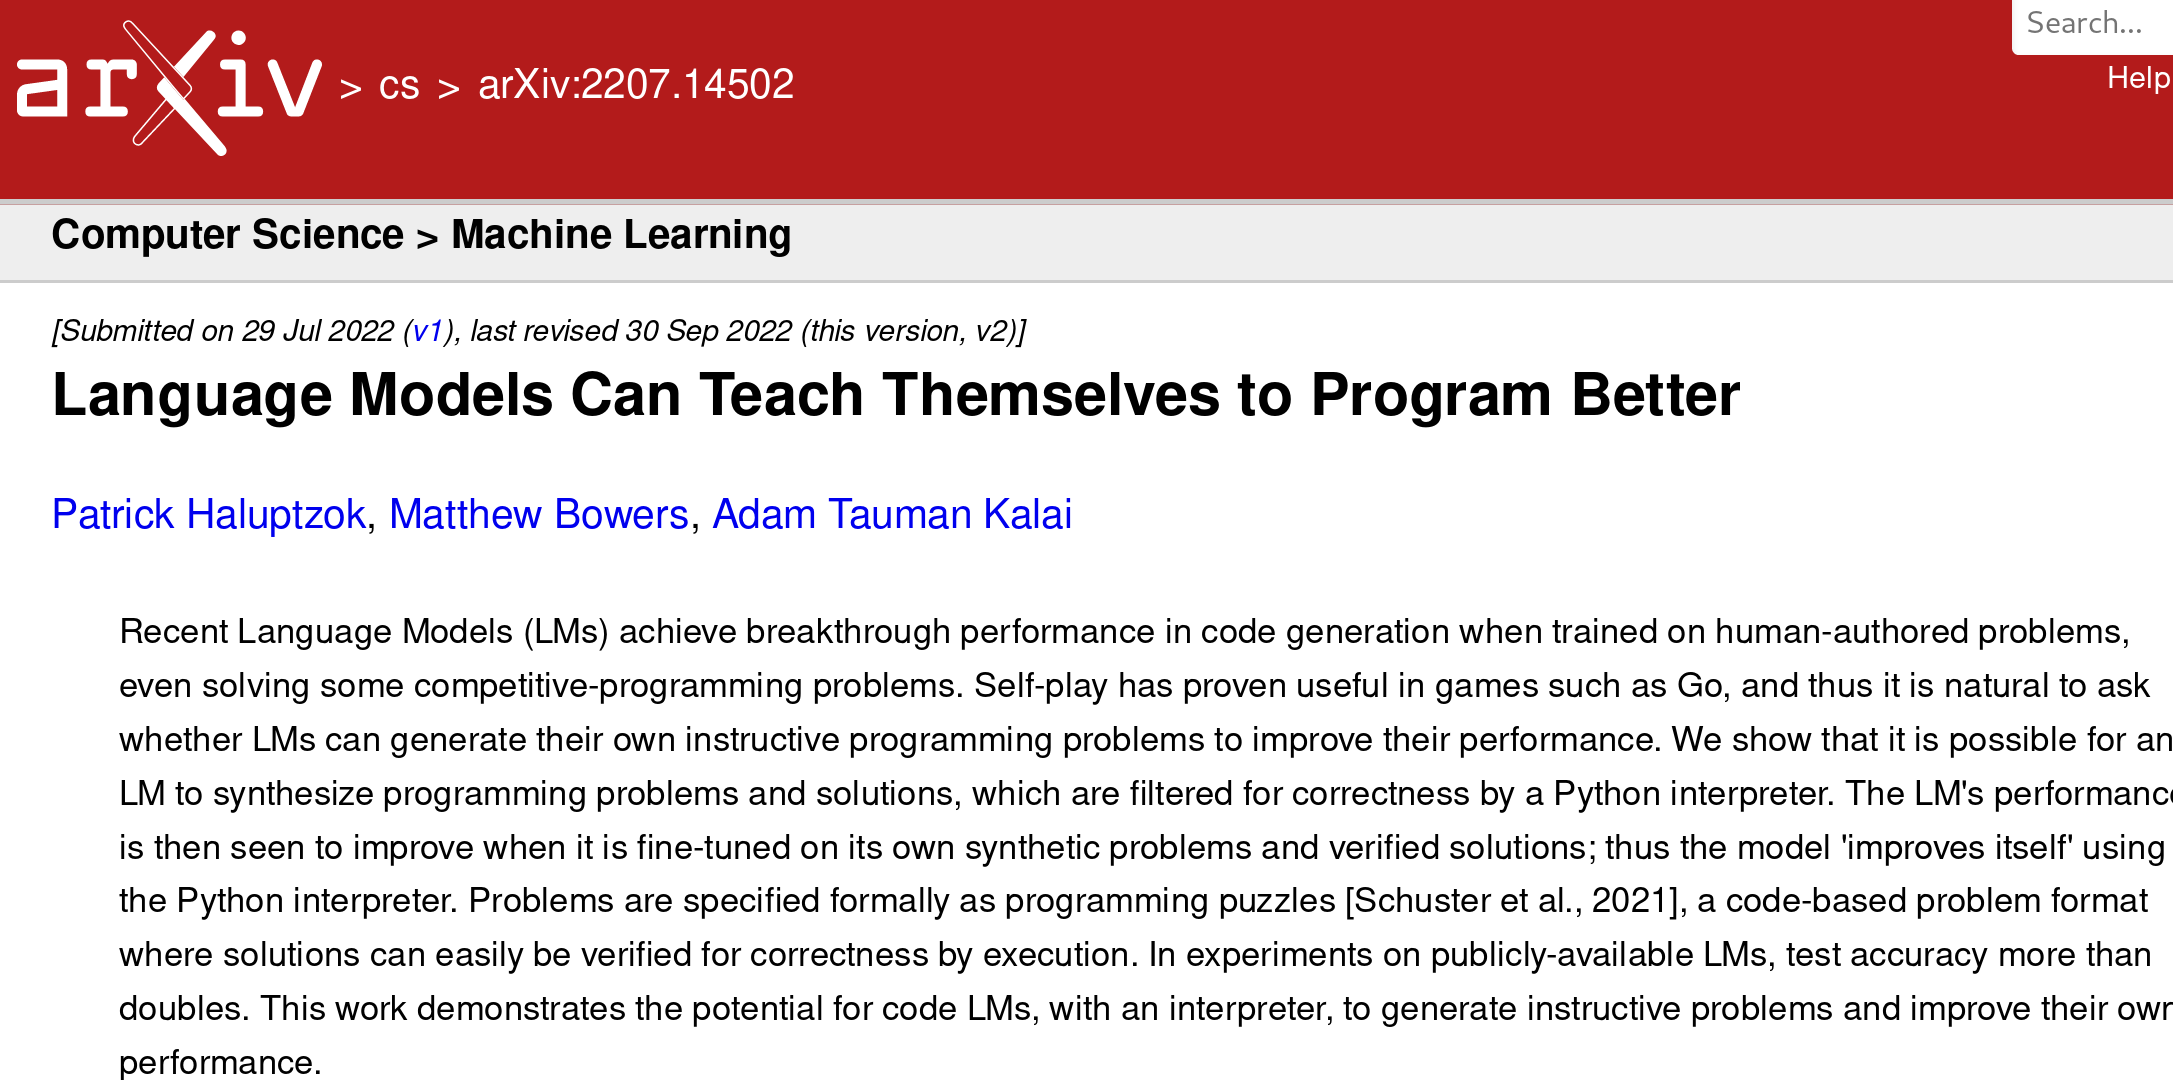
\includegraphics[width=10cm]{figs/llm-programming-better}
  \end{center}

  \begin{flushright}
    {\small
      \url{https://arxiv.org/abs/2207.14502}
    }
  \end{flushright}
  
\end{frame}

%%-----------------------------------------
\begin{frame}[fragile]
  \frametitle{Programming}

  \begin{center}
    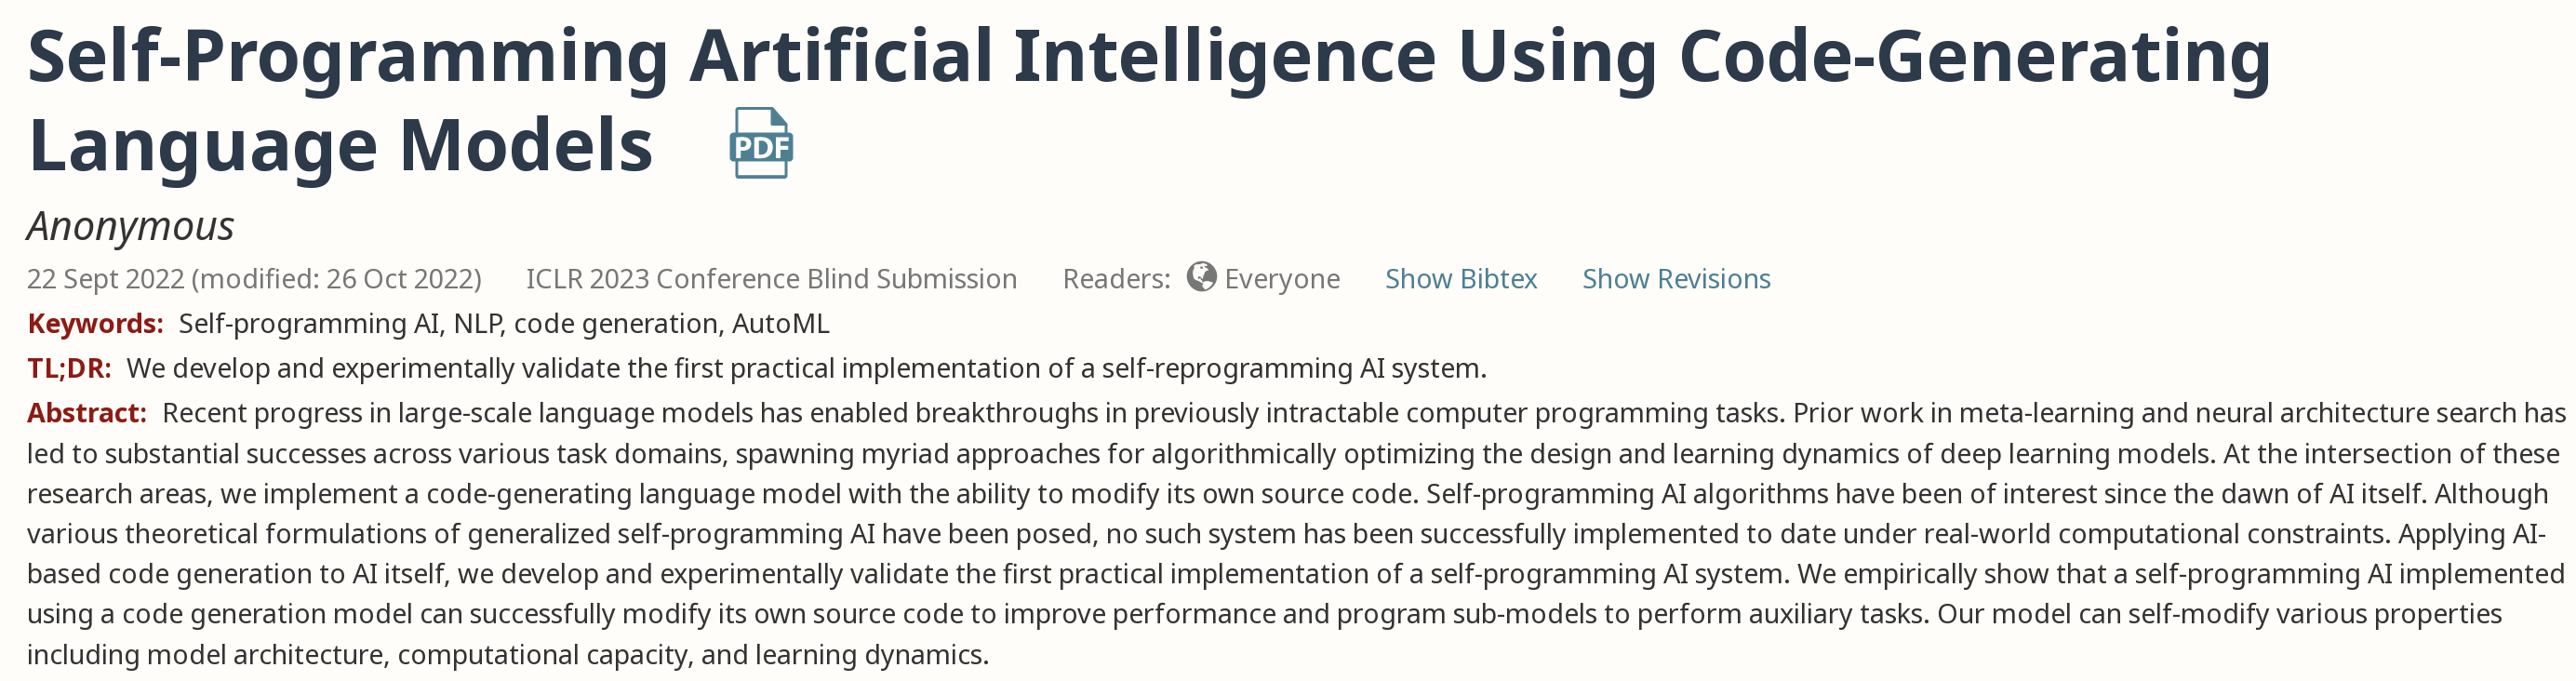
\includegraphics[width=10cm]{figs/self-programming}
  \end{center}

  \begin{flushright}
    {\scriptsize
      \url{https://keras.io/examples/generative/random_walks_with_stable_diffusion/}
    }
  \end{flushright}
  
\end{frame}




%%-----------------------------------------
%%-----------------------------------------
\section{Summarizing}

%% -----------------------------------------
\begin{frame}[fragile]

  {\Large \bf
    The future just started
  }
\end{frame}

%%-----------------------------------------
%%-----------------------------------------
\section*{References}

% -----------------------------------------
\begin{frame}[fragile]

  {\huge References, credits, license}
\end{frame}

%%-----------------------------------------
\begin{frame}[fragile]
%  \frametitle{References}

  {\small
    \begin{itemize}
    \item Transformers-Tutorials \\
      {\scriptsize \url{https://github.com/NielsRogge/Transformers-Tutorials}}
    \item Vision Transformers \\
      {\scriptsize \url{https://cameronrwolfe.substack.com/p/vision-transformers}}
    \item A walk through latent space with Stable Diffusion \\
      {\scriptsize \url{https://keras.io/examples/generative/random_walks_with_stable_diffusion/}}
    \item How Open Source is eating AI \\
      {\scriptsize \url{https://lspace.swyx.io/p/open-source-ai}}
    \end{itemize}
  }  
\end{frame}

%% -----------------------------------------
\begin{frame}[fragile]
%  \frametitle{References}


  {\small
    \begin{itemize}
    \item Awesome Diffusion Models \\
      {\scriptsize \url{https://github.com/heejkoo/Awesome-Diffusion-Models}}
    \item /r/StableDiffusion at Reddit \\
      {\scriptsize \url{https://www.reddit.com/r/StableDiffusion}}
    \item The Generative Landscape (WiP course) \\
      {\scriptsize \url{https://johnowhitaker.github.io/tglcourse/}}
    \end{itemize}
  }  
\end{frame}


% -----------------------------------------
\begin{frame}[fragile]
  \frametitle{Credits}

  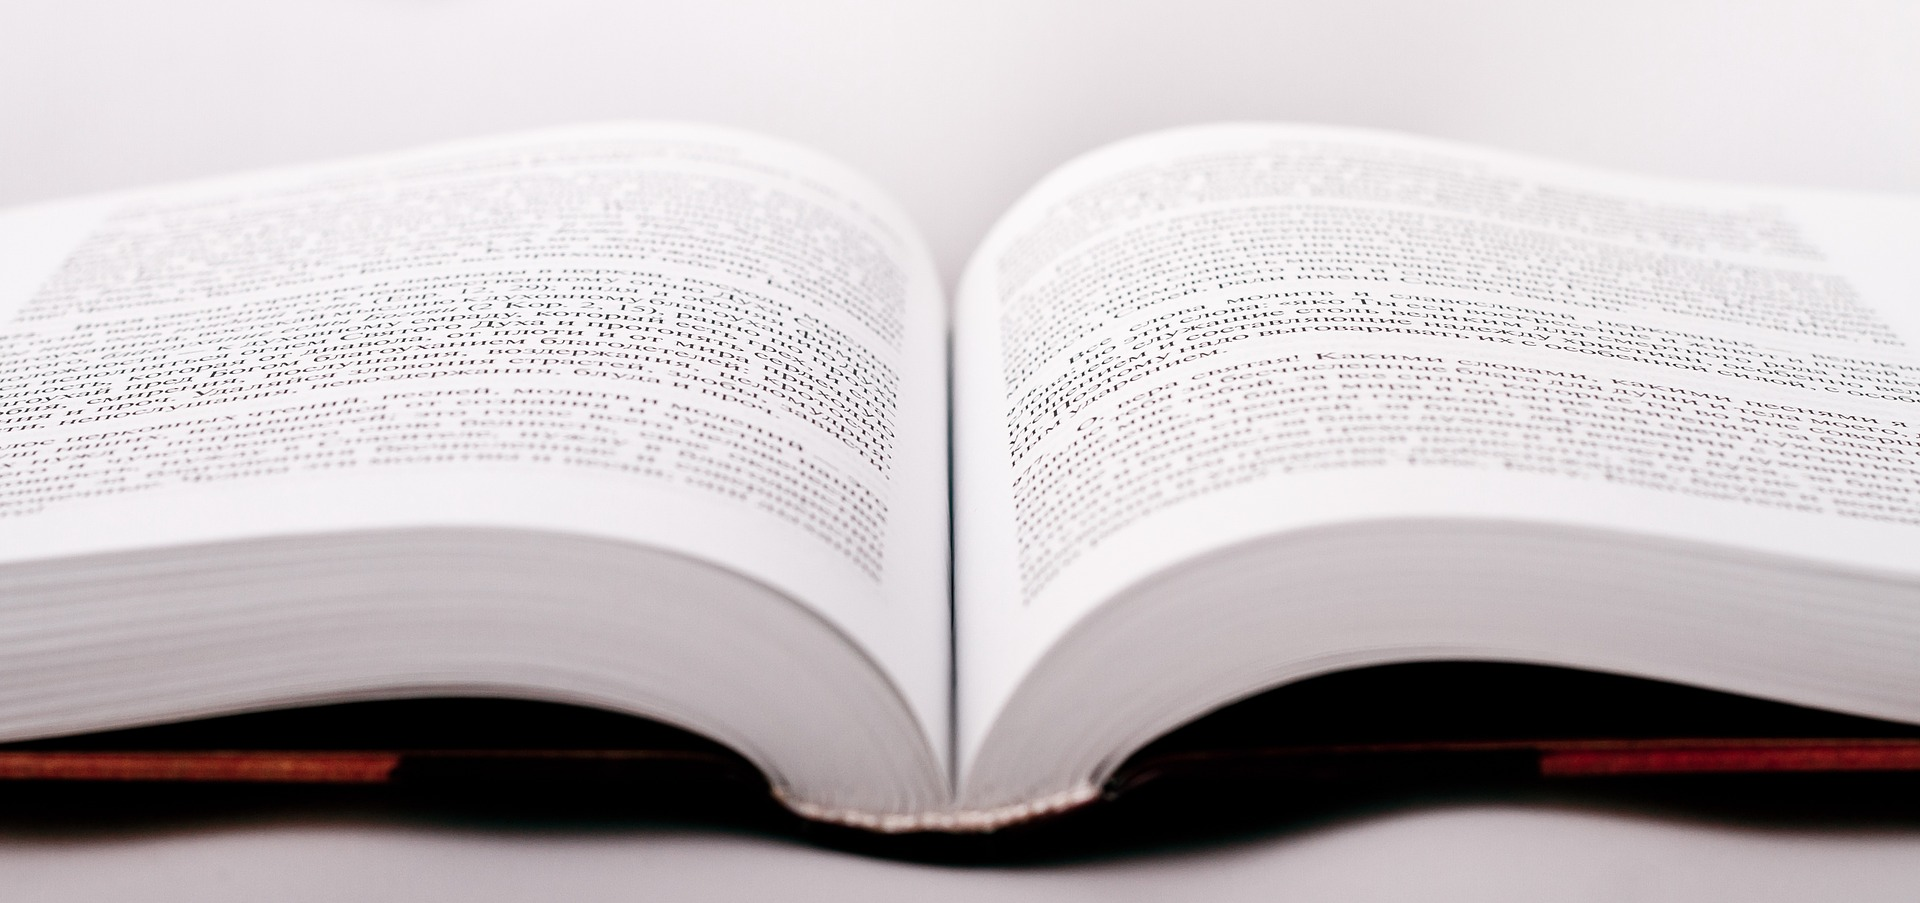
\includegraphics[width=1.5cm]{figs/bookpages}
  {\small \href{https://pixabay.com/en/book-reading-library-literature-1261800/}{Book}, by NikolayFrolochkin, Pixabay. \\ License: Creative Commons CC0\\}

\end{frame}



\frame{
~
\vspace{1cm}

\begin{flushright}


\includegraphics[width=2.2cm]{figs/by-sa}
 \\

\begin{footnotesize}
\copyright 2022-2023 Jesus M. Gonzalez-Barahona. \\

\vspace{.4cm}

Some rights reserved. This document is distributed under the terms of the Creative Commons License ``Attribution-ShareAlike 4.0'',
available in \\
{\scriptsize \url{http://creativecommons.org/licenses/by-sa/4.0/}} \\

\vspace{.4cm}

This document (including source) is available from
\url{https://jgbarah.github.io/presentations}

\end{footnotesize}
\end{flushright}

}
%%

%\againframe{firstframe}

\end{document}

%%% Local Variables:
%%% mode: latex
%%% TeX-master: t
%%% End:
